\documentclass[1p]{elsarticle_modified}
%\bibliographystyle{elsarticle-num}

%\usepackage[colorlinks]{hyperref}
%\usepackage{abbrmath_seonhwa} %\Abb, \Ascr, \Acal ,\Abf, \Afrak
\usepackage{amsfonts}
\usepackage{amssymb}
\usepackage{amsmath}
\usepackage{amsthm}
\usepackage{scalefnt}
\usepackage{amsbsy}
\usepackage{kotex}
\usepackage{caption}
\usepackage{subfig}
\usepackage{color}
\usepackage{graphicx}
\usepackage{xcolor} %% white, black, red, green, blue, cyan, magenta, yellow
\usepackage{float}
\usepackage{setspace}
\usepackage{hyperref}

\usepackage{tikz}
\usetikzlibrary{arrows}

\usepackage{multirow}
\usepackage{array} % fixed length table
\usepackage{hhline}

%%%%%%%%%%%%%%%%%%%%%
\makeatletter
\renewcommand*\env@matrix[1][\arraystretch]{%
	\edef\arraystretch{#1}%
	\hskip -\arraycolsep
	\let\@ifnextchar\new@ifnextchar
	\array{*\c@MaxMatrixCols c}}
\makeatother %https://tex.stackexchange.com/questions/14071/how-can-i-increase-the-line-spacing-in-a-matrix
%%%%%%%%%%%%%%%

\usepackage[normalem]{ulem}

\newcommand{\msout}[1]{\ifmmode\text{\sout{\ensuremath{#1}}}\else\sout{#1}\fi}
%SOURCE: \msout is \stkout macro in https://tex.stackexchange.com/questions/20609/strikeout-in-math-mode

\newcommand{\cancel}[1]{
	\ifmmode
	{\color{red}\msout{#1}}
	\else
	{\color{red}\sout{#1}}
	\fi
}

\newcommand{\add}[1]{
	{\color{blue}\uwave{#1}}
}

\newcommand{\replace}[2]{
	\ifmmode
	{\color{red}\msout{#1}}{\color{blue}\uwave{#2}}
	\else
	{\color{red}\sout{#1}}{\color{blue}\uwave{#2}}
	\fi
}

\newcommand{\Sol}{\mathcal{S}} %segment
\newcommand{\D}{D} %diagram
\newcommand{\A}{\mathcal{A}} %arc


%%%%%%%%%%%%%%%%%%%%%%%%%%%%%5 test

\def\sl{\operatorname{\textup{SL}}(2,\Cbb)}
\def\psl{\operatorname{\textup{PSL}}(2,\Cbb)}
\def\quan{\mkern 1mu \triangleright \mkern 1mu}

\theoremstyle{definition}
\newtheorem{thm}{Theorem}[section]
\newtheorem{prop}[thm]{Proposition}
\newtheorem{lem}[thm]{Lemma}
\newtheorem{ques}[thm]{Question}
\newtheorem{cor}[thm]{Corollary}
\newtheorem{defn}[thm]{Definition}
\newtheorem{exam}[thm]{Example}
\newtheorem{rmk}[thm]{Remark}
\newtheorem{alg}[thm]{Algorithm}

\newcommand{\I}{\sqrt{-1}}
\begin{document}

%\begin{frontmatter}
%
%\title{Boundary parabolic representations of knots up to 8 crossings}
%
%%% Group authors per affiliation:
%\author{Yunhi Cho} 
%\address{Department of Mathematics, University of Seoul, Seoul, Korea}
%\ead{yhcho@uos.ac.kr}
%
%
%\author{Seonhwa Kim} %\fnref{s_kim}}
%\address{Center for Geometry and Physics, Institute for Basic Science, Pohang, 37673, Korea}
%\ead{ryeona17@ibs.re.kr}
%
%\author{Hyuk Kim}
%\address{Department of Mathematical Sciences, Seoul National University, Seoul 08826, Korea}
%\ead{hyukkim@snu.ac.kr}
%
%\author{Seokbeom Yoon}
%\address{Department of Mathematical Sciences, Seoul National University, Seoul, 08826,  Korea}
%\ead{sbyoon15@snu.ac.kr}
%
%\begin{abstract}
%We find all boundary parabolic representation of knots up to 8 crossings.
%
%\end{abstract}
%\begin{keyword}
%    \MSC[2010] 57M25 
%\end{keyword}
%
%\end{frontmatter}

%\linenumbers
%\tableofcontents
%
\newcommand\colored[1]{\textcolor{white}{\rule[-0.35ex]{0.8em}{1.4ex}}\kern-0.8em\color{red} #1}%
%\newcommand\colored[1]{\textcolor{white}{ #1}\kern-2.17ex	\textcolor{white}{ #1}\kern-1.81ex	\textcolor{white}{ #1}\kern-2.15ex\color{red}#1	}

{\Large $\underline{12a_{0893}~(K12a_{0893})}$}

\setlength{\tabcolsep}{10pt}
\renewcommand{\arraystretch}{1.6}
\vspace{1cm}\begin{tabular}{m{100pt}>{\centering\arraybackslash}m{274pt}}
\multirow{5}{120pt}{
	\centering
	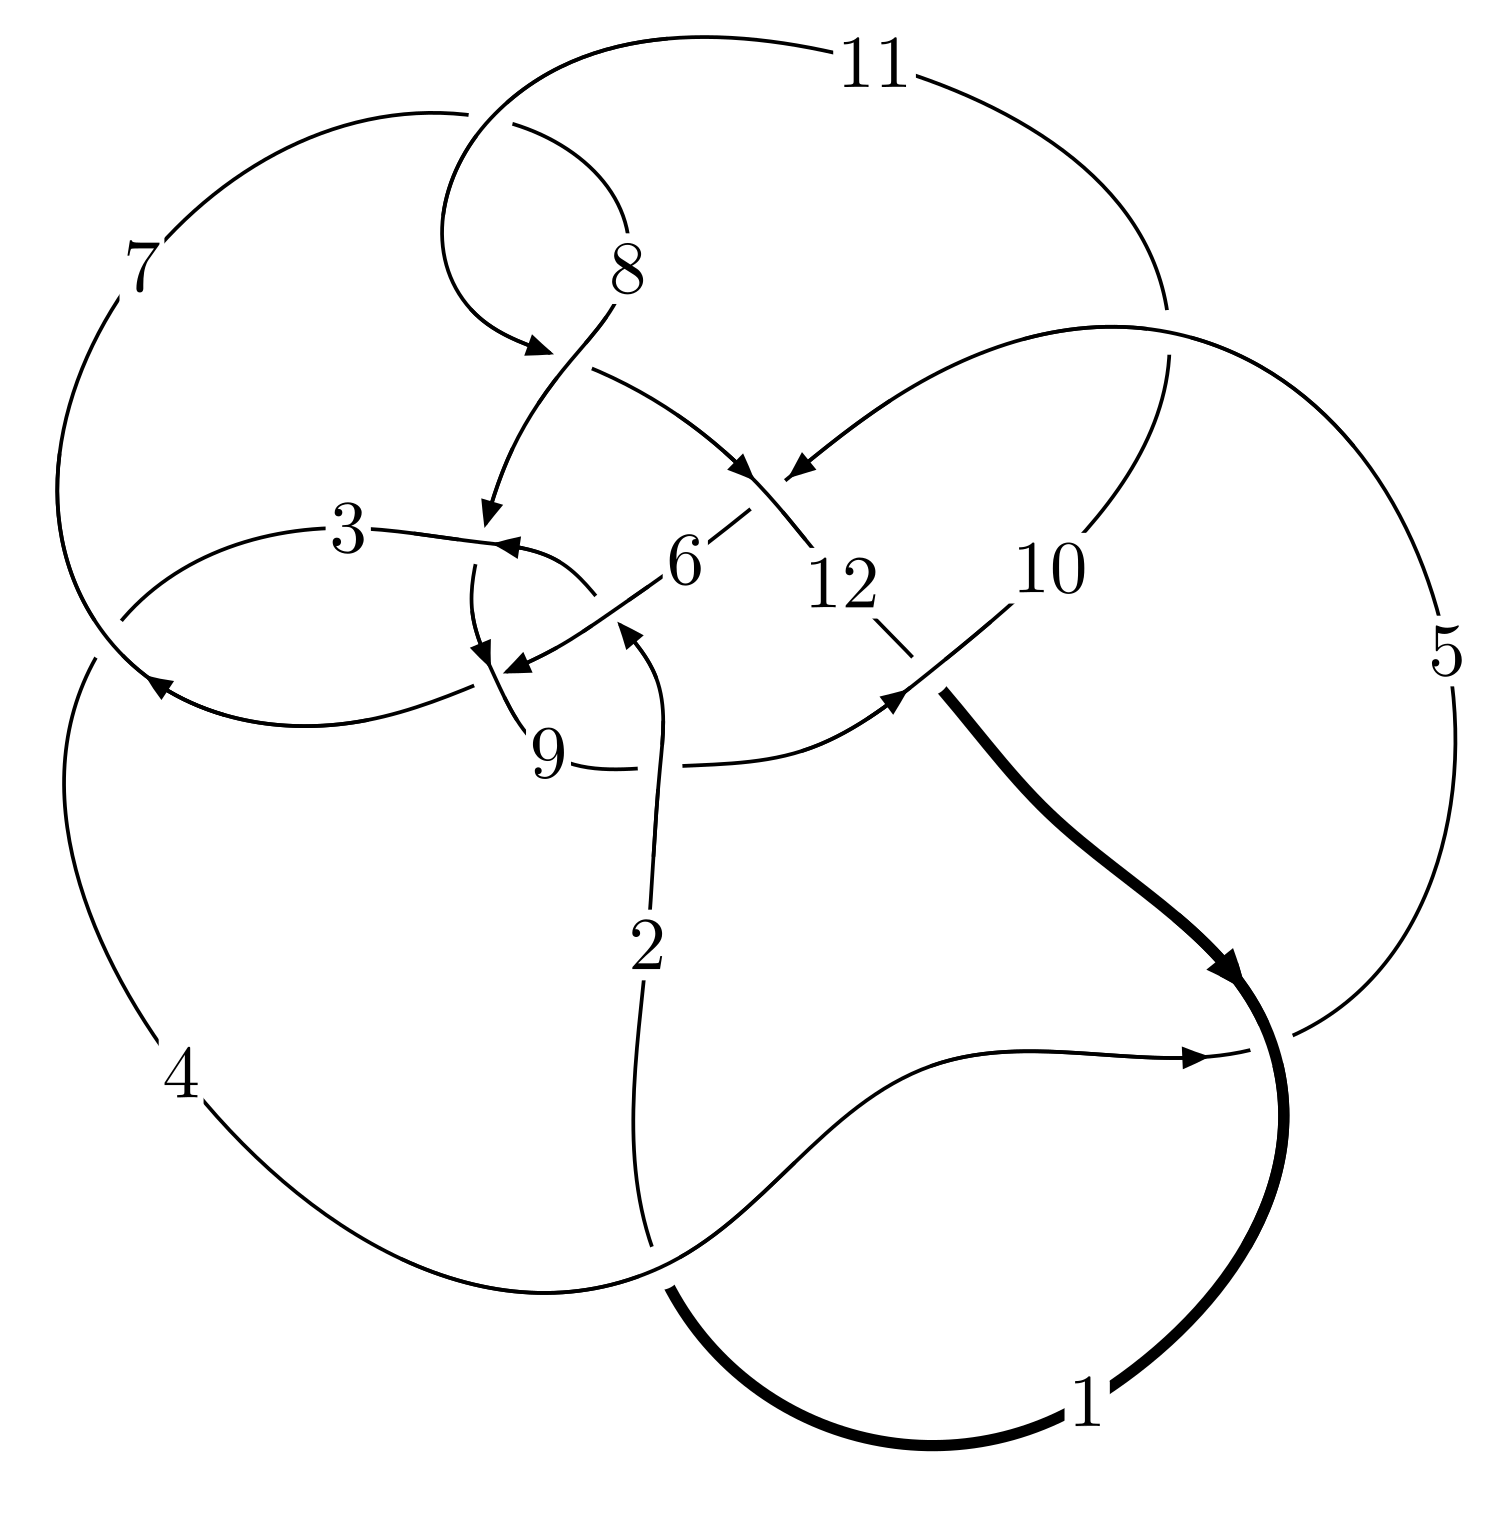
\includegraphics[width=112pt]{../../../GIT/diagram.site/Diagrams/png/1694_12a_0893.png}\\
\ \ \ A knot diagram\footnotemark}&
\allowdisplaybreaks
\textbf{Linearized knot diagam} \\
\cline{2-2}
 &
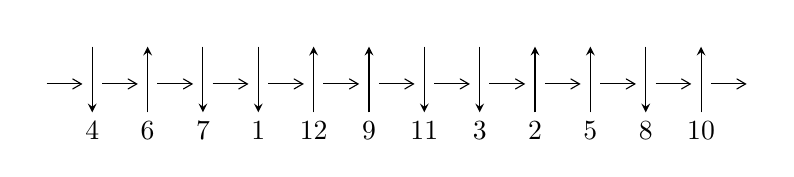
\begin{tikzpicture}[x=20pt, y=17pt]
	% nodes
	\node (C0) at (0, 0) {};
	\node (C1) at (1, 0) {};
	\node (C1U) at (1, +1) {};
	\node (C1D) at (1, -1) {4};

	\node (C2) at (2, 0) {};
	\node (C2U) at (2, +1) {};
	\node (C2D) at (2, -1) {6};

	\node (C3) at (3, 0) {};
	\node (C3U) at (3, +1) {};
	\node (C3D) at (3, -1) {7};

	\node (C4) at (4, 0) {};
	\node (C4U) at (4, +1) {};
	\node (C4D) at (4, -1) {1};

	\node (C5) at (5, 0) {};
	\node (C5U) at (5, +1) {};
	\node (C5D) at (5, -1) {12};

	\node (C6) at (6, 0) {};
	\node (C6U) at (6, +1) {};
	\node (C6D) at (6, -1) {9};

	\node (C7) at (7, 0) {};
	\node (C7U) at (7, +1) {};
	\node (C7D) at (7, -1) {11};

	\node (C8) at (8, 0) {};
	\node (C8U) at (8, +1) {};
	\node (C8D) at (8, -1) {3};

	\node (C9) at (9, 0) {};
	\node (C9U) at (9, +1) {};
	\node (C9D) at (9, -1) {2};

	\node (C10) at (10, 0) {};
	\node (C10U) at (10, +1) {};
	\node (C10D) at (10, -1) {5};

	\node (C11) at (11, 0) {};
	\node (C11U) at (11, +1) {};
	\node (C11D) at (11, -1) {8};

	\node (C12) at (12, 0) {};
	\node (C12U) at (12, +1) {};
	\node (C12D) at (12, -1) {10};
	\node (C13) at (13, 0) {};

	% arrows
	\draw[->,>={angle 60}]
	(C0) edge (C1) (C1) edge (C2) (C2) edge (C3) (C3) edge (C4) (C4) edge (C5) (C5) edge (C6) (C6) edge (C7) (C7) edge (C8) (C8) edge (C9) (C9) edge (C10) (C10) edge (C11) (C11) edge (C12) (C12) edge (C13) ;	\draw[->,>=stealth]
	(C1U) edge (C1D) (C2D) edge (C2U) (C3U) edge (C3D) (C4U) edge (C4D) (C5D) edge (C5U) (C6D) edge (C6U) (C7U) edge (C7D) (C8U) edge (C8D) (C9D) edge (C9U) (C10D) edge (C10U) (C11U) edge (C11D) (C12D) edge (C12U) ;
	\end{tikzpicture} \\
\hhline{~~} \\& 
\textbf{Solving Sequence} \\ \cline{2-2} 
 &
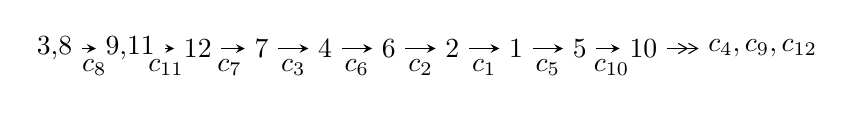
\begin{tikzpicture}[x=23pt, y=7pt]
	% node
	\node (A0) at (-1/8, 0) {3,8};
	\node (A1) at (17/16, 0) {9,11};
	\node (A2) at (17/8, 0) {12};
	\node (A3) at (25/8, 0) {7};
	\node (A4) at (33/8, 0) {4};
	\node (A5) at (41/8, 0) {6};
	\node (A6) at (49/8, 0) {2};
	\node (A7) at (57/8, 0) {1};
	\node (A8) at (65/8, 0) {5};
	\node (A9) at (73/8, 0) {10};
	\node (C1) at (1/2, -1) {$c_{8}$};
	\node (C2) at (13/8, -1) {$c_{11}$};
	\node (C3) at (21/8, -1) {$c_{7}$};
	\node (C4) at (29/8, -1) {$c_{3}$};
	\node (C5) at (37/8, -1) {$c_{6}$};
	\node (C6) at (45/8, -1) {$c_{2}$};
	\node (C7) at (53/8, -1) {$c_{1}$};
	\node (C8) at (61/8, -1) {$c_{5}$};
	\node (C9) at (69/8, -1) {$c_{10}$};
	\node (A10) at (11, 0) {$c_{4},c_{9},c_{12}$};

	% edge
	\draw[->,>=stealth]	
	(A0) edge (A1) (A1) edge (A2) (A2) edge (A3) (A3) edge (A4) (A4) edge (A5) (A5) edge (A6) (A6) edge (A7) (A7) edge (A8) (A8) edge (A9) ;
	\draw[->>,>={angle 60}]	
	(A9) edge (A10);
\end{tikzpicture} \\ 

\end{tabular} \\

\footnotetext{
The image of knot diagram is generated by the software ``\textbf{Draw programme}" developed by Andrew Bartholomew(\url{http://www.layer8.co.uk/maths/draw/index.htm\#Running-draw}), where we modified some parts for our purpose(\url{https://github.com/CATsTAILs/LinksPainter}).
}\phantom \\ \newline 
\centering \textbf{Ideals for irreducible components\footnotemark of $X_{\text{par}}$} 
 
\begin{align*}
I^u_{1}&=\langle 
-5.61103\times10^{2633} u^{209}-1.17812\times10^{2634} u^{208}+\cdots+2.36542\times10^{2634} b+2.70080\times10^{2633},\\
\phantom{I^u_{1}}&\phantom{= \langle  }6.58387\times10^{2634} u^{209}+1.29409\times10^{2635} u^{208}+\cdots+2.36542\times10^{2634} a-3.74081\times10^{2635},\\
\phantom{I^u_{1}}&\phantom{= \langle  }3 u^{210}+6 u^{209}+\cdots-26 u+1\rangle \\
I^u_{2}&=\langle 
1.26412\times10^{171} u^{55}-3.51118\times10^{171} u^{54}+\cdots+2.84952\times10^{170} b-1.69933\times10^{171},\\
\phantom{I^u_{2}}&\phantom{= \langle  }3.45571\times10^{170} u^{55}-9.11636\times10^{170} u^{54}+\cdots+2.84952\times10^{170} a+1.97333\times10^{170},\;3 u^{56}-9 u^{55}+\cdots-7 u+1\rangle \\
\\
\end{align*}
\raggedright * 2 irreducible components of $\dim_{\mathbb{C}}=0$, with total 266 representations.\\
\footnotetext{All coefficients of polynomials are rational numbers. But the coefficients are sometimes approximated in decimal forms when there is not enough margin.}
\newpage
\renewcommand{\arraystretch}{1}
\centering \section*{I. $I^u_{1}= \langle -5.61\times10^{2633} u^{209}-1.18\times10^{2634} u^{208}+\cdots+2.37\times10^{2634} b+2.70\times10^{2633},\;6.58\times10^{2634} u^{209}+1.29\times10^{2635} u^{208}+\cdots+2.37\times10^{2634} a-3.74\times10^{2635},\;3 u^{210}+6 u^{209}+\cdots-26 u+1 \rangle$}
\flushleft \textbf{(i) Arc colorings}\\
\begin{tabular}{m{7pt} m{180pt} m{7pt} m{180pt} }
\flushright $a_{3}=$&$\begin{pmatrix}0\\u\end{pmatrix}$ \\
\flushright $a_{8}=$&$\begin{pmatrix}1\\0\end{pmatrix}$ \\
\flushright $a_{9}=$&$\begin{pmatrix}1\\u^2\end{pmatrix}$ \\
\flushright $a_{11}=$&$\begin{pmatrix}-2.78338 u^{209}-5.47088 u^{208}+\cdots-408.910 u+15.8146\\0.237211 u^{209}+0.498058 u^{208}+\cdots+26.8040 u-0.114179\end{pmatrix}$ \\
\flushright $a_{12}=$&$\begin{pmatrix}-3.02059 u^{209}-5.96893 u^{208}+\cdots-435.714 u+15.9288\\0.237211 u^{209}+0.498058 u^{208}+\cdots+26.8040 u-0.114179\end{pmatrix}$ \\
\flushright $a_{7}=$&$\begin{pmatrix}1.17133 u^{209}+2.28236 u^{208}+\cdots+251.317 u-19.4374\\-0.336848 u^{209}-0.679864 u^{208}+\cdots-45.5636 u+1.65715\end{pmatrix}$ \\
\flushright $a_{4}=$&$\begin{pmatrix}-0.0423068 u^{209}-0.230676 u^{208}+\cdots+68.9630 u-11.9556\\-0.159705 u^{209}-0.320978 u^{208}+\cdots-26.1963 u+1.32984\end{pmatrix}$ \\
\flushright $a_{6}=$&$\begin{pmatrix}1.48273 u^{209}+2.90344 u^{208}+\cdots+295.968 u-21.0744\\-0.336339 u^{209}-0.680440 u^{208}+\cdots-45.6823 u+1.65772\end{pmatrix}$ \\
\flushright $a_{2}=$&$\begin{pmatrix}0.235422 u^{209}+0.325882 u^{208}+\cdots+124.375 u-14.6092\\-0.176154 u^{209}-0.345408 u^{208}+\cdots-29.8021 u+1.42071\end{pmatrix}$ \\
\flushright $a_{1}=$&$\begin{pmatrix}2.43638 u^{209}+4.77805 u^{208}+\cdots+340.373 u-14.4855\\-0.238536 u^{209}-0.486428 u^{208}+\cdots-26.9801 u+0.410462\end{pmatrix}$ \\
\flushright $a_{5}=$&$\begin{pmatrix}-0.272076 u^{209}-0.664735 u^{208}+\cdots-26.7015 u+0.929693\\0.00207036 u^{209}+0.00307822 u^{208}+\cdots+0.0551708 u+0.101753\end{pmatrix}$ \\
\flushright $a_{10}=$&$\begin{pmatrix}-2.23770 u^{209}-4.46873 u^{208}+\cdots-371.192 u+13.8781\\0.196187 u^{209}+0.405338 u^{208}+\cdots+25.3540 u-0.160323\end{pmatrix}$\\&\end{tabular}
\flushleft \textbf{(ii) Obstruction class $= -1$}\\~\\
\flushleft \textbf{(iii) Cusp Shapes $= -0.435971 u^{209}-0.805405 u^{208}+\cdots+121.187 u-8.89267$}\\~\\
\newpage\renewcommand{\arraystretch}{1}
\flushleft \textbf{(iv) u-Polynomials at the component}\newline \\
\begin{tabular}{m{50pt}|m{274pt}}
Crossings & \hspace{64pt}u-Polynomials at each crossing \\
\hline $$\begin{aligned}c_{1},c_{4}\end{aligned}$$&$\begin{aligned}
&u^{210}+10 u^{209}+\cdots-27478849 u+12092767
\end{aligned}$\\
\hline $$\begin{aligned}c_{2}\end{aligned}$$&$\begin{aligned}
&u^{210}-6 u^{209}+\cdots+49 u+1
\end{aligned}$\\
\hline $$\begin{aligned}c_{3}\end{aligned}$$&$\begin{aligned}
&u^{210}+8 u^{208}+\cdots+257055 u+4092
\end{aligned}$\\
\hline $$\begin{aligned}c_{5}\end{aligned}$$&$\begin{aligned}
&u^{210}+7 u^{209}+\cdots+1508984076 u+44022057
\end{aligned}$\\
\hline $$\begin{aligned}c_{6}\end{aligned}$$&$\begin{aligned}
&u^{210}+12 u^{209}+\cdots+4260 u+237
\end{aligned}$\\
\hline $$\begin{aligned}c_{7},c_{11}\end{aligned}$$&$\begin{aligned}
&u^{210}+2 u^{209}+\cdots-101779 u+358027
\end{aligned}$\\
\hline $$\begin{aligned}c_{8}\end{aligned}$$&$\begin{aligned}
&3(3 u^{210}+6 u^{209}+\cdots-26 u+1)
\end{aligned}$\\
\hline $$\begin{aligned}c_{9}\end{aligned}$$&$\begin{aligned}
&3(3 u^{210}-3 u^{209}+\cdots+4592789 u+999482)
\end{aligned}$\\
\hline $$\begin{aligned}c_{10}\end{aligned}$$&$\begin{aligned}
&3(3 u^{210}+15 u^{209}+\cdots+1.12391\times10^{8} u+1.34206\times10^{7})
\end{aligned}$\\
\hline $$\begin{aligned}c_{12}\end{aligned}$$&$\begin{aligned}
&u^{210}+12 u^{209}+\cdots+450 u+375
\end{aligned}$\\
\hline
\end{tabular}\\~\\
\newpage\renewcommand{\arraystretch}{1}
\flushleft \textbf{(v) Riley Polynomials at the component}\newline \\
\begin{tabular}{m{50pt}|m{274pt}}
Crossings & \hspace{64pt}Riley Polynomials at each crossing \\
\hline $$\begin{aligned}c_{1},c_{4}\end{aligned}$$&$\begin{aligned}
&y^{210}+148 y^{209}+\cdots+7967626144440991 y+146235013716289
\end{aligned}$\\
\hline $$\begin{aligned}c_{2}\end{aligned}$$&$\begin{aligned}
&y^{210}+22 y^{209}+\cdots+49 y+1
\end{aligned}$\\
\hline $$\begin{aligned}c_{3}\end{aligned}$$&$\begin{aligned}
&y^{210}+16 y^{209}+\cdots-23452087521 y+16744464
\end{aligned}$\\
\hline $$\begin{aligned}c_{5}\end{aligned}$$&$\begin{aligned}
&y^{210}+21 y^{209}+\cdots+183177916340579052 y+1937941502511249
\end{aligned}$\\
\hline $$\begin{aligned}c_{6}\end{aligned}$$&$\begin{aligned}
&y^{210}+8 y^{209}+\cdots+4428546 y+56169
\end{aligned}$\\
\hline $$\begin{aligned}c_{7},c_{11}\end{aligned}$$&$\begin{aligned}
&y^{210}-102 y^{209}+\cdots-7529227423575 y+128183332729
\end{aligned}$\\
\hline $$\begin{aligned}c_{8}\end{aligned}$$&$\begin{aligned}
&9(9 y^{210}+96 y^{209}+\cdots+290 y+1)
\end{aligned}$\\
\hline $$\begin{aligned}c_{9}\end{aligned}$$&$\begin{aligned}
&9(9 y^{210}+537 y^{209}+\cdots-2.72232\times10^{14} y+9.98964\times10^{11})
\end{aligned}$\\
\hline $$\begin{aligned}c_{10}\end{aligned}$$&$\begin{aligned}
&9\\
&\cdot(9 y^{210}-525 y^{209}+\cdots-18148003448693073 y+180112826454544)
\end{aligned}$\\
\hline $$\begin{aligned}c_{12}\end{aligned}$$&$\begin{aligned}
&y^{210}-34 y^{209}+\cdots-9502500 y+140625
\end{aligned}$\\
\hline
\end{tabular}\\~\\
\newpage\flushleft \textbf{(vi) Complex Volumes and Cusp Shapes}
$$\begin{array}{c|c|c}  
\text{Solutions to }I^u_{1}& \I (\text{vol} + \sqrt{-1}CS) & \text{Cusp shape}\\
 \hline 
\begin{aligned}
u &= \phantom{-}0.838294 + 0.540054 I \\
a &= \phantom{-}1.77803 - 0.11287 I \\
b &= \phantom{-}1.350600 + 0.028259 I\end{aligned}
 & -7.00637 - 2.65784 I & \phantom{-0.000000 } 0 \\ \hline\begin{aligned}
u &= \phantom{-}0.838294 - 0.540054 I \\
a &= \phantom{-}1.77803 + 0.11287 I \\
b &= \phantom{-}1.350600 - 0.028259 I\end{aligned}
 & -7.00637 + 2.65784 I & \phantom{-0.000000 } 0 \\ \hline\begin{aligned}
u &= -0.974110 + 0.329203 I \\
a &= \phantom{-}0.302974 + 0.036436 I \\
b &= \phantom{-}0.27482 - 1.51050 I\end{aligned}
 & \phantom{-}3.01434 + 4.31771 I & \phantom{-0.000000 } 0 \\ \hline\begin{aligned}
u &= -0.974110 - 0.329203 I \\
a &= \phantom{-}0.302974 - 0.036436 I \\
b &= \phantom{-}0.27482 + 1.51050 I\end{aligned}
 & \phantom{-}3.01434 - 4.31771 I & \phantom{-0.000000 } 0 \\ \hline\begin{aligned}
u &= -0.502020 + 0.818598 I \\
a &= \phantom{-}0.310752 - 1.345780 I \\
b &= -0.906972 + 0.145337 I\end{aligned}
 & -0.39504 + 4.95163 I & \phantom{-0.000000 } 0 \\ \hline\begin{aligned}
u &= -0.502020 - 0.818598 I \\
a &= \phantom{-}0.310752 + 1.345780 I \\
b &= -0.906972 - 0.145337 I\end{aligned}
 & -0.39504 - 4.95163 I & \phantom{-0.000000 } 0 \\ \hline\begin{aligned}
u &= -0.631212 + 0.704469 I \\
a &= \phantom{-}1.122220 + 0.782606 I \\
b &= -0.212816 - 0.811223 I\end{aligned}
 & \phantom{-}4.13252 + 1.14382 I & \phantom{-0.000000 } 0 \\ \hline\begin{aligned}
u &= -0.631212 - 0.704469 I \\
a &= \phantom{-}1.122220 - 0.782606 I \\
b &= -0.212816 + 0.811223 I\end{aligned}
 & \phantom{-}4.13252 - 1.14382 I & \phantom{-0.000000 } 0 \\ \hline\begin{aligned}
u &= \phantom{-}0.299721 + 0.889161 I \\
a &= \phantom{-}0.06887 + 1.80152 I \\
b &= -1.137400 - 0.557002 I\end{aligned}
 & \phantom{-}1.50993 - 6.12543 I & \phantom{-0.000000 } 0 \\ \hline\begin{aligned}
u &= \phantom{-}0.299721 - 0.889161 I \\
a &= \phantom{-}0.06887 - 1.80152 I \\
b &= -1.137400 + 0.557002 I\end{aligned}
 & \phantom{-}1.50993 + 6.12543 I & \phantom{-0.000000 } 0\\
 \hline 
 \end{array}$$\newpage$$\begin{array}{c|c|c}  
\text{Solutions to }I^u_{1}& \I (\text{vol} + \sqrt{-1}CS) & \text{Cusp shape}\\
 \hline 
\begin{aligned}
u &= \phantom{-}0.932725 + 0.048673 I \\
a &= \phantom{-}2.30883 + 0.48865 I \\
b &= \phantom{-}1.072620 + 0.492248 I\end{aligned}
 & -4.49722 - 5.58626 I & \phantom{-0.000000 } 0 \\ \hline\begin{aligned}
u &= \phantom{-}0.932725 - 0.048673 I \\
a &= \phantom{-}2.30883 - 0.48865 I \\
b &= \phantom{-}1.072620 - 0.492248 I\end{aligned}
 & -4.49722 + 5.58626 I & \phantom{-0.000000 } 0 \\ \hline\begin{aligned}
u &= -0.975344 + 0.442624 I \\
a &= -1.11120 - 1.12254 I \\
b &= -0.959846 - 0.255558 I\end{aligned}
 & -3.94127 + 2.23313 I & \phantom{-0.000000 } 0 \\ \hline\begin{aligned}
u &= -0.975344 - 0.442624 I \\
a &= -1.11120 + 1.12254 I \\
b &= -0.959846 + 0.255558 I\end{aligned}
 & -3.94127 - 2.23313 I & \phantom{-0.000000 } 0 \\ \hline\begin{aligned}
u &= -0.561718 + 0.923956 I \\
a &= -0.574246 - 0.849632 I \\
b &= -0.899775 + 0.623859 I\end{aligned}
 & \phantom{-}1.71023 + 4.27980 I & \phantom{-0.000000 } 0 \\ \hline\begin{aligned}
u &= -0.561718 - 0.923956 I \\
a &= -0.574246 + 0.849632 I \\
b &= -0.899775 - 0.623859 I\end{aligned}
 & \phantom{-}1.71023 - 4.27980 I & \phantom{-0.000000 } 0 \\ \hline\begin{aligned}
u &= -0.910592 + 0.588984 I \\
a &= -2.11961 - 0.21354 I \\
b &= -1.114550 + 0.369861 I\end{aligned}
 & -3.23520 + 7.08529 I & \phantom{-0.000000 } 0 \\ \hline\begin{aligned}
u &= -0.910592 - 0.588984 I \\
a &= -2.11961 + 0.21354 I \\
b &= -1.114550 - 0.369861 I\end{aligned}
 & -3.23520 - 7.08529 I & \phantom{-0.000000 } 0 \\ \hline\begin{aligned}
u &= \phantom{-}0.602104 + 0.902630 I \\
a &= \phantom{-}0.352390 + 0.985041 I \\
b &= -0.676345 + 0.160093 I\end{aligned}
 & -1.28161 - 4.61716 I & \phantom{-0.000000 } 0 \\ \hline\begin{aligned}
u &= \phantom{-}0.602104 - 0.902630 I \\
a &= \phantom{-}0.352390 - 0.985041 I \\
b &= -0.676345 - 0.160093 I\end{aligned}
 & -1.28161 + 4.61716 I & \phantom{-0.000000 } 0\\
 \hline 
 \end{array}$$\newpage$$\begin{array}{c|c|c}  
\text{Solutions to }I^u_{1}& \I (\text{vol} + \sqrt{-1}CS) & \text{Cusp shape}\\
 \hline 
\begin{aligned}
u &= \phantom{-}0.794512 + 0.745220 I \\
a &= -0.0260919 - 0.1248450 I \\
b &= \phantom{-}0.098483 + 1.091630 I\end{aligned}
 & \phantom{-}2.07212 - 7.26772 I & \phantom{-0.000000 } 0 \\ \hline\begin{aligned}
u &= \phantom{-}0.794512 - 0.745220 I \\
a &= -0.0260919 + 0.1248450 I \\
b &= \phantom{-}0.098483 - 1.091630 I\end{aligned}
 & \phantom{-}2.07212 + 7.26772 I & \phantom{-0.000000 } 0 \\ \hline\begin{aligned}
u &= \phantom{-}0.882397 + 0.218865 I \\
a &= -2.41669 - 0.21438 I \\
b &= -1.076990 - 0.277729 I\end{aligned}
 & -4.24696 - 3.56604 I & \phantom{-0.000000 } 0 \\ \hline\begin{aligned}
u &= \phantom{-}0.882397 - 0.218865 I \\
a &= -2.41669 + 0.21438 I \\
b &= -1.076990 + 0.277729 I\end{aligned}
 & -4.24696 + 3.56604 I & \phantom{-0.000000 } 0 \\ \hline\begin{aligned}
u &= -1.077580 + 0.192610 I \\
a &= \phantom{-}1.063200 + 0.208572 I \\
b &= \phantom{-}1.51413 - 0.32222 I\end{aligned}
 & -2.95365 - 1.10457 I & \phantom{-0.000000 } 0 \\ \hline\begin{aligned}
u &= -1.077580 - 0.192610 I \\
a &= \phantom{-}1.063200 - 0.208572 I \\
b &= \phantom{-}1.51413 + 0.32222 I\end{aligned}
 & -2.95365 + 1.10457 I & \phantom{-0.000000 } 0 \\ \hline\begin{aligned}
u &= \phantom{-}0.883763 + 0.193908 I \\
a &= \phantom{-}0.915880 - 0.288558 I \\
b &= \phantom{-}1.289470 + 0.457581 I\end{aligned}
 & -2.85438 + 0.37294 I & \phantom{-0.000000 } 0 \\ \hline\begin{aligned}
u &= \phantom{-}0.883763 - 0.193908 I \\
a &= \phantom{-}0.915880 + 0.288558 I \\
b &= \phantom{-}1.289470 - 0.457581 I\end{aligned}
 & -2.85438 - 0.37294 I & \phantom{-0.000000 } 0 \\ \hline\begin{aligned}
u &= \phantom{-}0.291081 + 0.846442 I \\
a &= \phantom{-}0.881435 - 0.399940 I \\
b &= -0.622853 + 0.669170 I\end{aligned}
 & \phantom{-}3.55993 - 0.33553 I & \phantom{-0.000000 } 0 \\ \hline\begin{aligned}
u &= \phantom{-}0.291081 - 0.846442 I \\
a &= \phantom{-}0.881435 + 0.399940 I \\
b &= -0.622853 - 0.669170 I\end{aligned}
 & \phantom{-}3.55993 + 0.33553 I & \phantom{-0.000000 } 0\\
 \hline 
 \end{array}$$\newpage$$\begin{array}{c|c|c}  
\text{Solutions to }I^u_{1}& \I (\text{vol} + \sqrt{-1}CS) & \text{Cusp shape}\\
 \hline 
\begin{aligned}
u &= -0.038123 + 1.104440 I \\
a &= \phantom{-}1.131140 + 0.040930 I \\
b &= -1.328670 - 0.120397 I\end{aligned}
 & \phantom{-}3.24826 - 0.03375 I & \phantom{-0.000000 } 0 \\ \hline\begin{aligned}
u &= -0.038123 - 1.104440 I \\
a &= \phantom{-}1.131140 - 0.040930 I \\
b &= -1.328670 + 0.120397 I\end{aligned}
 & \phantom{-}3.24826 + 0.03375 I & \phantom{-0.000000 } 0 \\ \hline\begin{aligned}
u &= -0.268475 + 1.072690 I \\
a &= \phantom{-}0.043255 - 0.398396 I \\
b &= -0.785143 + 0.405357 I\end{aligned}
 & \phantom{-}1.50142 + 3.76427 I & \phantom{-0.000000 } 0 \\ \hline\begin{aligned}
u &= -0.268475 - 1.072690 I \\
a &= \phantom{-}0.043255 + 0.398396 I \\
b &= -0.785143 - 0.405357 I\end{aligned}
 & \phantom{-}1.50142 - 3.76427 I & \phantom{-0.000000 } 0 \\ \hline\begin{aligned}
u &= \phantom{-}0.142639 + 1.103720 I \\
a &= \phantom{-}0.306795 - 0.176767 I \\
b &= -0.526898 - 0.279012 I\end{aligned}
 & \phantom{-}6.06903 + 0.32205 I & \phantom{-0.000000 } 0 \\ \hline\begin{aligned}
u &= \phantom{-}0.142639 - 1.103720 I \\
a &= \phantom{-}0.306795 + 0.176767 I \\
b &= -0.526898 + 0.279012 I\end{aligned}
 & \phantom{-}6.06903 - 0.32205 I & \phantom{-0.000000 } 0 \\ \hline\begin{aligned}
u &= -0.806291 + 0.362257 I \\
a &= \phantom{-}1.224860 + 0.178142 I \\
b &= \phantom{-}1.27334 - 0.93876 I\end{aligned}
 & -0.52426 + 3.89742 I & \phantom{-0.000000 } 0 \\ \hline\begin{aligned}
u &= -0.806291 - 0.362257 I \\
a &= \phantom{-}1.224860 - 0.178142 I \\
b &= \phantom{-}1.27334 + 0.93876 I\end{aligned}
 & -0.52426 - 3.89742 I & \phantom{-0.000000 } 0 \\ \hline\begin{aligned}
u &= \phantom{-}0.352923 + 0.810416 I \\
a &= -0.665121 - 0.292336 I \\
b &= -0.881282 + 0.748614 I\end{aligned}
 & \phantom{-}1.79631 + 0.92582 I & \phantom{-0.000000 } 0 \\ \hline\begin{aligned}
u &= \phantom{-}0.352923 - 0.810416 I \\
a &= -0.665121 + 0.292336 I \\
b &= -0.881282 - 0.748614 I\end{aligned}
 & \phantom{-}1.79631 - 0.92582 I & \phantom{-0.000000 } 0\\
 \hline 
 \end{array}$$\newpage$$\begin{array}{c|c|c}  
\text{Solutions to }I^u_{1}& \I (\text{vol} + \sqrt{-1}CS) & \text{Cusp shape}\\
 \hline 
\begin{aligned}
u &= -0.861574 + 0.729370 I \\
a &= -2.19323 - 0.96284 I \\
b &= -0.565584 + 0.608098 I\end{aligned}
 & \phantom{-}5.01219 + 8.07894 I & \phantom{-0.000000 } 0 \\ \hline\begin{aligned}
u &= -0.861574 - 0.729370 I \\
a &= -2.19323 + 0.96284 I \\
b &= -0.565584 - 0.608098 I\end{aligned}
 & \phantom{-}5.01219 - 8.07894 I & \phantom{-0.000000 } 0 \\ \hline\begin{aligned}
u &= -1.129100 + 0.140684 I \\
a &= -1.23791 - 0.89091 I \\
b &= -0.810907 + 0.540868 I\end{aligned}
 & \phantom{-}0.28583 + 6.27248 I & \phantom{-0.000000 } 0 \\ \hline\begin{aligned}
u &= -1.129100 - 0.140684 I \\
a &= -1.23791 + 0.89091 I \\
b &= -0.810907 - 0.540868 I\end{aligned}
 & \phantom{-}0.28583 - 6.27248 I & \phantom{-0.000000 } 0 \\ \hline\begin{aligned}
u &= -0.206487 + 0.835219 I \\
a &= -1.60062 - 1.85574 I \\
b &= -0.576402 - 0.135329 I\end{aligned}
 & \phantom{-}1.13788 - 6.73057 I & \phantom{-0.000000 } 0 \\ \hline\begin{aligned}
u &= -0.206487 - 0.835219 I \\
a &= -1.60062 + 1.85574 I \\
b &= -0.576402 + 0.135329 I\end{aligned}
 & \phantom{-}1.13788 + 6.73057 I & \phantom{-0.000000 } 0 \\ \hline\begin{aligned}
u &= \phantom{-}0.956158 + 0.628238 I \\
a &= -1.83593 + 0.38440 I \\
b &= -1.234210 - 0.338031 I\end{aligned}
 & -4.47132 - 5.17456 I & \phantom{-0.000000 } 0 \\ \hline\begin{aligned}
u &= \phantom{-}0.956158 - 0.628238 I \\
a &= -1.83593 - 0.38440 I \\
b &= -1.234210 + 0.338031 I\end{aligned}
 & -4.47132 + 5.17456 I & \phantom{-0.000000 } 0 \\ \hline\begin{aligned}
u &= \phantom{-}0.761568 + 0.874361 I \\
a &= -0.185779 + 0.940016 I \\
b &= \phantom{-}0.281809 - 0.549412 I\end{aligned}
 & -1.99263 + 2.64285 I & \phantom{-0.000000 } 0 \\ \hline\begin{aligned}
u &= \phantom{-}0.761568 - 0.874361 I \\
a &= -0.185779 - 0.940016 I \\
b &= \phantom{-}0.281809 + 0.549412 I\end{aligned}
 & -1.99263 - 2.64285 I & \phantom{-0.000000 } 0\\
 \hline 
 \end{array}$$\newpage$$\begin{array}{c|c|c}  
\text{Solutions to }I^u_{1}& \I (\text{vol} + \sqrt{-1}CS) & \text{Cusp shape}\\
 \hline 
\begin{aligned}
u &= -0.665830 + 0.949582 I \\
a &= -0.216448 + 0.192004 I \\
b &= \phantom{-}0.925219 + 0.649865 I\end{aligned}
 & \phantom{-}1.28817 + 1.13940 I & \phantom{-0.000000 } 0 \\ \hline\begin{aligned}
u &= -0.665830 - 0.949582 I \\
a &= -0.216448 - 0.192004 I \\
b &= \phantom{-}0.925219 - 0.649865 I\end{aligned}
 & \phantom{-}1.28817 - 1.13940 I & \phantom{-0.000000 } 0 \\ \hline\begin{aligned}
u &= \phantom{-}0.282254 + 1.131240 I \\
a &= -1.10347 + 1.66886 I \\
b &= -0.761673 - 0.275295 I\end{aligned}
 & -2.76953 - 0.36673 I & \phantom{-0.000000 } 0 \\ \hline\begin{aligned}
u &= \phantom{-}0.282254 - 1.131240 I \\
a &= -1.10347 - 1.66886 I \\
b &= -0.761673 + 0.275295 I\end{aligned}
 & -2.76953 + 0.36673 I & \phantom{-0.000000 } 0 \\ \hline\begin{aligned}
u &= -0.513702 + 1.048320 I \\
a &= \phantom{-}0.933452 + 0.478499 I \\
b &= \phantom{-}0.852363 - 0.218931 I\end{aligned}
 & -1.69340 + 1.74417 I & \phantom{-0.000000 } 0 \\ \hline\begin{aligned}
u &= -0.513702 - 1.048320 I \\
a &= \phantom{-}0.933452 - 0.478499 I \\
b &= \phantom{-}0.852363 + 0.218931 I\end{aligned}
 & -1.69340 - 1.74417 I & \phantom{-0.000000 } 0 \\ \hline\begin{aligned}
u &= -0.556498 + 0.618059 I \\
a &= -1.37127 - 0.60951 I \\
b &= -1.32437 + 0.77348 I\end{aligned}
 & \phantom{-}0.86117 + 13.48710 I & \phantom{-0.000000 } 0 \\ \hline\begin{aligned}
u &= -0.556498 - 0.618059 I \\
a &= -1.37127 + 0.60951 I \\
b &= -1.32437 - 0.77348 I\end{aligned}
 & \phantom{-}0.86117 - 13.48710 I & \phantom{-0.000000 } 0 \\ \hline\begin{aligned}
u &= \phantom{-}0.499885 + 0.663782 I \\
a &= -1.44798 + 0.85498 I \\
b &= -1.254670 - 0.634309 I\end{aligned}
 & -2.50988 - 8.05345 I & \phantom{-0.000000 } 0 \\ \hline\begin{aligned}
u &= \phantom{-}0.499885 - 0.663782 I \\
a &= -1.44798 - 0.85498 I \\
b &= -1.254670 + 0.634309 I\end{aligned}
 & -2.50988 + 8.05345 I & \phantom{-0.000000 } 0\\
 \hline 
 \end{array}$$\newpage$$\begin{array}{c|c|c}  
\text{Solutions to }I^u_{1}& \I (\text{vol} + \sqrt{-1}CS) & \text{Cusp shape}\\
 \hline 
\begin{aligned}
u &= \phantom{-}0.805967 + 0.177860 I \\
a &= \phantom{-}0.434459 + 0.646256 I \\
b &= -0.146359 - 0.254865 I\end{aligned}
 & \phantom{-}0.95657 + 3.34017 I & \phantom{-0.000000 } 0 \\ \hline\begin{aligned}
u &= \phantom{-}0.805967 - 0.177860 I \\
a &= \phantom{-}0.434459 - 0.646256 I \\
b &= -0.146359 + 0.254865 I\end{aligned}
 & \phantom{-}0.95657 - 3.34017 I & \phantom{-0.000000 } 0 \\ \hline\begin{aligned}
u &= -0.730148 + 0.325441 I \\
a &= \phantom{-}0.689403 + 0.803956 I \\
b &= \phantom{-}0.248934 + 0.487387 I\end{aligned}
 & -2.34065 + 1.51221 I & \phantom{-0.000000 } 0 \\ \hline\begin{aligned}
u &= -0.730148 - 0.325441 I \\
a &= \phantom{-}0.689403 - 0.803956 I \\
b &= \phantom{-}0.248934 - 0.487387 I\end{aligned}
 & -2.34065 - 1.51221 I & \phantom{-0.000000 } 0 \\ \hline\begin{aligned}
u &= \phantom{-}0.082067 + 0.789063 I \\
a &= -2.51671 - 0.30100 I \\
b &= \phantom{-}0.700472 - 0.136876 I\end{aligned}
 & \phantom{-}4.67674 + 2.13623 I & \phantom{-0.000000 } 0 \\ \hline\begin{aligned}
u &= \phantom{-}0.082067 - 0.789063 I \\
a &= -2.51671 + 0.30100 I \\
b &= \phantom{-}0.700472 + 0.136876 I\end{aligned}
 & \phantom{-}4.67674 - 2.13623 I & \phantom{-0.000000 } 0 \\ \hline\begin{aligned}
u &= -0.396844 + 0.672747 I \\
a &= \phantom{-}0.477507 - 0.394204 I \\
b &= \phantom{-}0.354193 - 0.256651 I\end{aligned}
 & -0.59462 + 1.63631 I & \phantom{-0.000000 } 0 \\ \hline\begin{aligned}
u &= -0.396844 - 0.672747 I \\
a &= \phantom{-}0.477507 + 0.394204 I \\
b &= \phantom{-}0.354193 + 0.256651 I\end{aligned}
 & -0.59462 - 1.63631 I & \phantom{-0.000000 } 0 \\ \hline\begin{aligned}
u &= \phantom{-}0.000149 + 0.779699 I \\
a &= -2.05632 - 0.40832 I \\
b &= \phantom{-}1.151910 + 0.441528 I\end{aligned}
 & \phantom{-}1.73719 - 11.11930 I & \phantom{-0.000000 } 0 \\ \hline\begin{aligned}
u &= \phantom{-}0.000149 - 0.779699 I \\
a &= -2.05632 + 0.40832 I \\
b &= \phantom{-}1.151910 - 0.441528 I\end{aligned}
 & \phantom{-}1.73719 + 11.11930 I & \phantom{-0.000000 } 0\\
 \hline 
 \end{array}$$\newpage$$\begin{array}{c|c|c}  
\text{Solutions to }I^u_{1}& \I (\text{vol} + \sqrt{-1}CS) & \text{Cusp shape}\\
 \hline 
\begin{aligned}
u &= \phantom{-}0.949273 + 0.771417 I \\
a &= \phantom{-}0.579696 - 0.324202 I \\
b &= \phantom{-}0.328331 + 1.185990 I\end{aligned}
 & \phantom{-}1.57222 - 4.42354 I & \phantom{-0.000000 } 0 \\ \hline\begin{aligned}
u &= \phantom{-}0.949273 - 0.771417 I \\
a &= \phantom{-}0.579696 + 0.324202 I \\
b &= \phantom{-}0.328331 - 1.185990 I\end{aligned}
 & \phantom{-}1.57222 + 4.42354 I & \phantom{-0.000000 } 0 \\ \hline\begin{aligned}
u &= \phantom{-}0.219917 + 1.206290 I \\
a &= -0.247126 + 0.003737 I \\
b &= -0.695623 - 0.473447 I\end{aligned}
 & \phantom{-}4.41442 - 9.47905 I & \phantom{-0.000000 } 0 \\ \hline\begin{aligned}
u &= \phantom{-}0.219917 - 1.206290 I \\
a &= -0.247126 - 0.003737 I \\
b &= -0.695623 + 0.473447 I\end{aligned}
 & \phantom{-}4.41442 + 9.47905 I & \phantom{-0.000000 } 0 \\ \hline\begin{aligned}
u &= -0.202107 + 0.740906 I \\
a &= -1.43945 + 0.88654 I \\
b &= \phantom{-}0.957278 - 0.420548 I\end{aligned}
 & -2.24052 + 6.62924 I & \phantom{-0.000000 } 0 \\ \hline\begin{aligned}
u &= -0.202107 - 0.740906 I \\
a &= -1.43945 - 0.88654 I \\
b &= \phantom{-}0.957278 + 0.420548 I\end{aligned}
 & -2.24052 - 6.62924 I & \phantom{-0.000000 } 0 \\ \hline\begin{aligned}
u &= -1.088940 + 0.577327 I \\
a &= \phantom{-}1.376260 + 0.191861 I \\
b &= \phantom{-}1.50735 + 0.08128 I\end{aligned}
 & -5.87042 - 1.91423 I & \phantom{-0.000000 } 0 \\ \hline\begin{aligned}
u &= -1.088940 - 0.577327 I \\
a &= \phantom{-}1.376260 - 0.191861 I \\
b &= \phantom{-}1.50735 - 0.08128 I\end{aligned}
 & -5.87042 + 1.91423 I & \phantom{-0.000000 } 0 \\ \hline\begin{aligned}
u &= -0.299101 + 0.694271 I \\
a &= \phantom{-}0.229867 - 0.239996 I \\
b &= \phantom{-}0.305748 - 0.639795 I\end{aligned}
 & -0.06110 + 1.78502 I & \phantom{-0.000000 } 0 \\ \hline\begin{aligned}
u &= -0.299101 - 0.694271 I \\
a &= \phantom{-}0.229867 + 0.239996 I \\
b &= \phantom{-}0.305748 + 0.639795 I\end{aligned}
 & -0.06110 - 1.78502 I & \phantom{-0.000000 } 0\\
 \hline 
 \end{array}$$\newpage$$\begin{array}{c|c|c}  
\text{Solutions to }I^u_{1}& \I (\text{vol} + \sqrt{-1}CS) & \text{Cusp shape}\\
 \hline 
\begin{aligned}
u &= -0.702449 + 0.275050 I \\
a &= \phantom{-}3.41512 + 0.46045 I \\
b &= \phantom{-}1.117660 - 0.549361 I\end{aligned}
 & -0.05361 + 11.89730 I & \phantom{-0.000000 } 0 \\ \hline\begin{aligned}
u &= -0.702449 - 0.275050 I \\
a &= \phantom{-}3.41512 - 0.46045 I \\
b &= \phantom{-}1.117660 + 0.549361 I\end{aligned}
 & -0.05361 - 11.89730 I & \phantom{-0.000000 } 0 \\ \hline\begin{aligned}
u &= -0.773109 + 0.976730 I \\
a &= -0.168386 - 0.112342 I \\
b &= -0.339086 - 0.627992 I\end{aligned}
 & -0.88491 + 4.23594 I & \phantom{-0.000000 } 0 \\ \hline\begin{aligned}
u &= -0.773109 - 0.976730 I \\
a &= -0.168386 + 0.112342 I \\
b &= -0.339086 + 0.627992 I\end{aligned}
 & -0.88491 - 4.23594 I & \phantom{-0.000000 } 0 \\ \hline\begin{aligned}
u &= -1.138080 + 0.558034 I \\
a &= -1.281100 - 0.010003 I \\
b &= -1.389430 - 0.120494 I\end{aligned}
 & -7.72543 + 5.67594 I & \phantom{-0.000000 } 0 \\ \hline\begin{aligned}
u &= -1.138080 - 0.558034 I \\
a &= -1.281100 + 0.010003 I \\
b &= -1.389430 + 0.120494 I\end{aligned}
 & -7.72543 - 5.67594 I & \phantom{-0.000000 } 0 \\ \hline\begin{aligned}
u &= -0.503915 + 0.527742 I \\
a &= \phantom{-}0.307213 + 0.874366 I \\
b &= \phantom{-}0.920430 - 0.907941 I\end{aligned}
 & -0.74677 + 6.77543 I & \phantom{-0.000000 } 0 \\ \hline\begin{aligned}
u &= -0.503915 - 0.527742 I \\
a &= \phantom{-}0.307213 - 0.874366 I \\
b &= \phantom{-}0.920430 + 0.907941 I\end{aligned}
 & -0.74677 - 6.77543 I & \phantom{-0.000000 } 0 \\ \hline\begin{aligned}
u &= \phantom{-}0.580935 + 1.145110 I \\
a &= \phantom{-}0.058772 - 0.156627 I \\
b &= -0.538663 + 0.798032 I\end{aligned}
 & \phantom{-}5.18100 - 1.10780 I & \phantom{-0.000000 } 0 \\ \hline\begin{aligned}
u &= \phantom{-}0.580935 - 1.145110 I \\
a &= \phantom{-}0.058772 + 0.156627 I \\
b &= -0.538663 - 0.798032 I\end{aligned}
 & \phantom{-}5.18100 + 1.10780 I & \phantom{-0.000000 } 0\\
 \hline 
 \end{array}$$\newpage$$\begin{array}{c|c|c}  
\text{Solutions to }I^u_{1}& \I (\text{vol} + \sqrt{-1}CS) & \text{Cusp shape}\\
 \hline 
\begin{aligned}
u &= -0.286489 + 0.647018 I \\
a &= -1.14375 - 2.69066 I \\
b &= -0.982337 + 0.550153 I\end{aligned}
 & \phantom{-}2.47295 + 5.07532 I & \phantom{-0.000000 } 0 \\ \hline\begin{aligned}
u &= -0.286489 - 0.647018 I \\
a &= -1.14375 + 2.69066 I \\
b &= -0.982337 - 0.550153 I\end{aligned}
 & \phantom{-}2.47295 - 5.07532 I & \phantom{-0.000000 } 0 \\ \hline\begin{aligned}
u &= \phantom{-}0.556103 + 0.432905 I \\
a &= -0.46178 - 1.70459 I \\
b &= \phantom{-}0.350612 - 0.679158 I\end{aligned}
 & \phantom{-}2.20453 - 7.10994 I & \phantom{-0.000000 } 0 \\ \hline\begin{aligned}
u &= \phantom{-}0.556103 - 0.432905 I \\
a &= -0.46178 + 1.70459 I \\
b &= \phantom{-}0.350612 + 0.679158 I\end{aligned}
 & \phantom{-}2.20453 + 7.10994 I & \phantom{-0.000000 } 0 \\ \hline\begin{aligned}
u &= \phantom{-}0.993146 + 0.878069 I \\
a &= \phantom{-}0.165270 - 0.243800 I \\
b &= -0.142644 + 1.176400 I\end{aligned}
 & \phantom{-}1.53849 - 3.99678 I & \phantom{-0.000000 } 0 \\ \hline\begin{aligned}
u &= \phantom{-}0.993146 - 0.878069 I \\
a &= \phantom{-}0.165270 + 0.243800 I \\
b &= -0.142644 - 1.176400 I\end{aligned}
 & \phantom{-}1.53849 + 3.99678 I & \phantom{-0.000000 } 0 \\ \hline\begin{aligned}
u &= \phantom{-}0.572408 + 1.196250 I \\
a &= -0.227683 + 0.056236 I \\
b &= \phantom{-}0.458780 - 0.414775 I\end{aligned}
 & \phantom{-}4.38891 - 8.29891 I & \phantom{-0.000000 } 0 \\ \hline\begin{aligned}
u &= \phantom{-}0.572408 - 1.196250 I \\
a &= -0.227683 - 0.056236 I \\
b &= \phantom{-}0.458780 + 0.414775 I\end{aligned}
 & \phantom{-}4.38891 + 8.29891 I & \phantom{-0.000000 } 0 \\ \hline\begin{aligned}
u &= \phantom{-}1.179300 + 0.610583 I \\
a &= -1.262920 + 0.190665 I \\
b &= -1.61506 - 0.03720 I\end{aligned}
 & -4.92707 - 10.37180 I & \phantom{-0.000000 } 0 \\ \hline\begin{aligned}
u &= \phantom{-}1.179300 - 0.610583 I \\
a &= -1.262920 - 0.190665 I \\
b &= -1.61506 + 0.03720 I\end{aligned}
 & -4.92707 + 10.37180 I & \phantom{-0.000000 } 0\\
 \hline 
 \end{array}$$\newpage$$\begin{array}{c|c|c}  
\text{Solutions to }I^u_{1}& \I (\text{vol} + \sqrt{-1}CS) & \text{Cusp shape}\\
 \hline 
\begin{aligned}
u &= -1.077930 + 0.785964 I \\
a &= -0.236627 + 0.217969 I \\
b &= -0.378843 - 1.139770 I\end{aligned}
 & \phantom{-}6.38657 + 5.55190 I & \phantom{-0.000000 } 0 \\ \hline\begin{aligned}
u &= -1.077930 - 0.785964 I \\
a &= -0.236627 - 0.217969 I \\
b &= -0.378843 + 1.139770 I\end{aligned}
 & \phantom{-}6.38657 - 5.55190 I & \phantom{-0.000000 } 0 \\ \hline\begin{aligned}
u &= -0.370481 + 0.533275 I \\
a &= \phantom{-}1.083500 + 0.849965 I \\
b &= \phantom{-}1.224680 - 0.380525 I\end{aligned}
 & -2.17764 + 1.67158 I & \phantom{-0.000000 } 0 \\ \hline\begin{aligned}
u &= -0.370481 - 0.533275 I \\
a &= \phantom{-}1.083500 - 0.849965 I \\
b &= \phantom{-}1.224680 + 0.380525 I\end{aligned}
 & -2.17764 - 1.67158 I & \phantom{-0.000000 } 0 \\ \hline\begin{aligned}
u &= -0.844209 + 1.057240 I \\
a &= \phantom{-}1.62430 + 0.88862 I \\
b &= \phantom{-}1.106270 - 0.464937 I\end{aligned}
 & \phantom{-}2.27330 + 12.13740 I & \phantom{-0.000000 } 0 \\ \hline\begin{aligned}
u &= -0.844209 - 1.057240 I \\
a &= \phantom{-}1.62430 - 0.88862 I \\
b &= \phantom{-}1.106270 + 0.464937 I\end{aligned}
 & \phantom{-}2.27330 - 12.13740 I & \phantom{-0.000000 } 0 \\ \hline\begin{aligned}
u &= -0.751764 + 1.131800 I \\
a &= -1.23605 - 1.06569 I \\
b &= -1.016700 + 0.677033 I\end{aligned}
 & \phantom{-}3.84639 + 6.58326 I & \phantom{-0.000000 } 0 \\ \hline\begin{aligned}
u &= -0.751764 - 1.131800 I \\
a &= -1.23605 + 1.06569 I \\
b &= -1.016700 - 0.677033 I\end{aligned}
 & \phantom{-}3.84639 - 6.58326 I & \phantom{-0.000000 } 0 \\ \hline\begin{aligned}
u &= \phantom{-}0.083256 + 0.621860 I \\
a &= -1.089660 + 0.209851 I \\
b &= -0.967510 - 0.795769 I\end{aligned}
 & \phantom{-}3.55279 + 4.63528 I & \phantom{-0.000000 } 0 \\ \hline\begin{aligned}
u &= \phantom{-}0.083256 - 0.621860 I \\
a &= -1.089660 - 0.209851 I \\
b &= -0.967510 + 0.795769 I\end{aligned}
 & \phantom{-}3.55279 - 4.63528 I & \phantom{-0.000000 } 0\\
 \hline 
 \end{array}$$\newpage$$\begin{array}{c|c|c}  
\text{Solutions to }I^u_{1}& \I (\text{vol} + \sqrt{-1}CS) & \text{Cusp shape}\\
 \hline 
\begin{aligned}
u &= -0.544266 + 1.290110 I \\
a &= \phantom{-}0.134657 - 0.191636 I \\
b &= \phantom{-}0.628070 + 0.270831 I\end{aligned}
 & \phantom{-}0.98489 + 1.78465 I & \phantom{-0.000000 } 0 \\ \hline\begin{aligned}
u &= -0.544266 - 1.290110 I \\
a &= \phantom{-}0.134657 + 0.191636 I \\
b &= \phantom{-}0.628070 - 0.270831 I\end{aligned}
 & \phantom{-}0.98489 - 1.78465 I & \phantom{-0.000000 } 0 \\ \hline\begin{aligned}
u &= \phantom{-}0.429507 + 0.407611 I \\
a &= \phantom{-}1.29030 - 0.96089 I \\
b &= \phantom{-}1.31815 + 0.63665 I\end{aligned}
 & -2.12743 - 4.25100 I & \phantom{-0.000000 } 0 \\ \hline\begin{aligned}
u &= \phantom{-}0.429507 - 0.407611 I \\
a &= \phantom{-}1.29030 + 0.96089 I \\
b &= \phantom{-}1.31815 - 0.63665 I\end{aligned}
 & -2.12743 + 4.25100 I & \phantom{-0.000000 } 0 \\ \hline\begin{aligned}
u &= \phantom{-}0.571298 + 0.140121 I \\
a &= \phantom{-}1.75453 - 0.00376 I \\
b &= \phantom{-}1.39662 + 0.64840 I\end{aligned}
 & -1.15203 - 2.71654 I & \phantom{-0.000000 } 0 \\ \hline\begin{aligned}
u &= \phantom{-}0.571298 - 0.140121 I \\
a &= \phantom{-}1.75453 + 0.00376 I \\
b &= \phantom{-}1.39662 - 0.64840 I\end{aligned}
 & -1.15203 + 2.71654 I & \phantom{-0.000000 } 0 \\ \hline\begin{aligned}
u &= \phantom{-}0.75235 + 1.19938 I \\
a &= \phantom{-}0.268695 + 0.266373 I \\
b &= -1.11748 + 0.92510 I\end{aligned}
 & \phantom{-}3.57512 - 2.37918 I & \phantom{-0.000000 } 0 \\ \hline\begin{aligned}
u &= \phantom{-}0.75235 - 1.19938 I \\
a &= \phantom{-}0.268695 - 0.266373 I \\
b &= -1.11748 - 0.92510 I\end{aligned}
 & \phantom{-}3.57512 + 2.37918 I & \phantom{-0.000000 } 0 \\ \hline\begin{aligned}
u &= -1.07753 + 0.92119 I \\
a &= \phantom{-}1.75661 + 0.51364 I \\
b &= \phantom{-}0.787113 - 0.392648 I\end{aligned}
 & \phantom{-}6.29350 + 0.71217 I & \phantom{-0.000000 } 0 \\ \hline\begin{aligned}
u &= -1.07753 - 0.92119 I \\
a &= \phantom{-}1.75661 - 0.51364 I \\
b &= \phantom{-}0.787113 + 0.392648 I\end{aligned}
 & \phantom{-}6.29350 - 0.71217 I & \phantom{-0.000000 } 0\\
 \hline 
 \end{array}$$\newpage$$\begin{array}{c|c|c}  
\text{Solutions to }I^u_{1}& \I (\text{vol} + \sqrt{-1}CS) & \text{Cusp shape}\\
 \hline 
\begin{aligned}
u &= \phantom{-}0.95245 + 1.05842 I \\
a &= -0.0593108 + 0.0983097 I \\
b &= \phantom{-}0.358476 - 1.008920 I\end{aligned}
 & -1.38946 - 9.53042 I & \phantom{-0.000000 } 0 \\ \hline\begin{aligned}
u &= \phantom{-}0.95245 - 1.05842 I \\
a &= -0.0593108 - 0.0983097 I \\
b &= \phantom{-}0.358476 + 1.008920 I\end{aligned}
 & -1.38946 + 9.53042 I & \phantom{-0.000000 } 0 \\ \hline\begin{aligned}
u &= -1.01245 + 1.02934 I \\
a &= -0.1044490 + 0.0090545 I \\
b &= \phantom{-}0.419459 + 1.221530 I\end{aligned}
 & \phantom{-}3.1418 + 15.2882 I & \phantom{-0.000000 } 0 \\ \hline\begin{aligned}
u &= -1.01245 - 1.02934 I \\
a &= -0.1044490 - 0.0090545 I \\
b &= \phantom{-}0.419459 - 1.221530 I\end{aligned}
 & \phantom{-}3.1418 - 15.2882 I & \phantom{-0.000000 } 0 \\ \hline\begin{aligned}
u &= \phantom{-}0.392570 + 0.385220 I \\
a &= \phantom{-}1.59506 - 1.60422 I \\
b &= \phantom{-}1.178910 + 0.632393 I\end{aligned}
 & -1.69409 - 3.94908 I & \phantom{-0.000000 } 0 \\ \hline\begin{aligned}
u &= \phantom{-}0.392570 - 0.385220 I \\
a &= \phantom{-}1.59506 + 1.60422 I \\
b &= \phantom{-}1.178910 - 0.632393 I\end{aligned}
 & -1.69409 + 3.94908 I & \phantom{-0.000000 } 0 \\ \hline\begin{aligned}
u &= -0.91619 + 1.12719 I \\
a &= -0.627803 - 0.956862 I \\
b &= \phantom{-}0.036746 + 0.921669 I\end{aligned}
 & \phantom{-}3.21822 - 7.78812 I & \phantom{-0.000000 } 0 \\ \hline\begin{aligned}
u &= -0.91619 - 1.12719 I \\
a &= -0.627803 + 0.956862 I \\
b &= \phantom{-}0.036746 - 0.921669 I\end{aligned}
 & \phantom{-}3.21822 + 7.78812 I & \phantom{-0.000000 } 0 \\ \hline\begin{aligned}
u &= \phantom{-}1.43287 + 0.29295 I \\
a &= -1.62321 - 0.46309 I \\
b &= -0.736511 + 0.089319 I\end{aligned}
 & -2.89131 - 3.41550 I & \phantom{-0.000000 } 0 \\ \hline\begin{aligned}
u &= \phantom{-}1.43287 - 0.29295 I \\
a &= -1.62321 + 0.46309 I \\
b &= -0.736511 - 0.089319 I\end{aligned}
 & -2.89131 + 3.41550 I & \phantom{-0.000000 } 0\\
 \hline 
 \end{array}$$\newpage$$\begin{array}{c|c|c}  
\text{Solutions to }I^u_{1}& \I (\text{vol} + \sqrt{-1}CS) & \text{Cusp shape}\\
 \hline 
\begin{aligned}
u &= \phantom{-}0.014909 + 0.531363 I \\
a &= \phantom{-}0.453187 + 0.029063 I \\
b &= -0.107859 - 1.004670 I\end{aligned}
 & \phantom{-}0.79385 + 2.10722 I & \phantom{-}8.15045 - 5.26873 I \\ \hline\begin{aligned}
u &= \phantom{-}0.014909 - 0.531363 I \\
a &= \phantom{-}0.453187 - 0.029063 I \\
b &= -0.107859 + 1.004670 I\end{aligned}
 & \phantom{-}0.79385 - 2.10722 I & \phantom{-}8.15045 + 5.26873 I \\ \hline\begin{aligned}
u &= -1.13983 + 0.92777 I \\
a &= \phantom{-}0.318709 - 0.032039 I \\
b &= -0.29566 - 1.68166 I\end{aligned}
 & \phantom{-}3.24679 + 4.68284 I & \phantom{-0.000000 } 0 \\ \hline\begin{aligned}
u &= -1.13983 - 0.92777 I \\
a &= \phantom{-}0.318709 + 0.032039 I \\
b &= -0.29566 + 1.68166 I\end{aligned}
 & \phantom{-}3.24679 - 4.68284 I & \phantom{-0.000000 } 0 \\ \hline\begin{aligned}
u &= \phantom{-}0.149898 + 0.472455 I \\
a &= -0.341742 + 0.540391 I \\
b &= \phantom{-}0.581439 + 0.999013 I\end{aligned}
 & \phantom{-}1.37894 - 4.54768 I & \phantom{-}6.26858 + 10.41405 I \\ \hline\begin{aligned}
u &= \phantom{-}0.149898 - 0.472455 I \\
a &= -0.341742 - 0.540391 I \\
b &= \phantom{-}0.581439 - 0.999013 I\end{aligned}
 & \phantom{-}1.37894 + 4.54768 I & \phantom{-}6.26858 - 10.41405 I \\ \hline\begin{aligned}
u &= \phantom{-}0.448268 + 0.195955 I \\
a &= -2.52717 + 3.05511 I \\
b &= -1.024250 - 0.392230 I\end{aligned}
 & -5.23201 - 1.19230 I & -14.5106 + 0. I\phantom{ +0.000000I} \\ \hline\begin{aligned}
u &= \phantom{-}0.448268 - 0.195955 I \\
a &= -2.52717 - 3.05511 I \\
b &= -1.024250 + 0.392230 I\end{aligned}
 & -5.23201 + 1.19230 I & -14.5106 + 0. I\phantom{ +0.000000I} \\ \hline\begin{aligned}
u &= -0.347392 + 0.342546 I \\
a &= \phantom{-}4.09657 + 1.43461 I \\
b &= \phantom{-}1.077110 - 0.450997 I\end{aligned}
 & \phantom{-}2.55963 + 0.63721 I & \phantom{-}3.86681 - 1.76840 I \\ \hline\begin{aligned}
u &= -0.347392 - 0.342546 I \\
a &= \phantom{-}4.09657 - 1.43461 I \\
b &= \phantom{-}1.077110 + 0.450997 I\end{aligned}
 & \phantom{-}2.55963 - 0.63721 I & \phantom{-}3.86681 + 1.76840 I\\
 \hline 
 \end{array}$$\newpage$$\begin{array}{c|c|c}  
\text{Solutions to }I^u_{1}& \I (\text{vol} + \sqrt{-1}CS) & \text{Cusp shape}\\
 \hline 
\begin{aligned}
u &= \phantom{-}0.95610 + 1.17232 I \\
a &= \phantom{-}1.46292 - 0.76538 I \\
b &= \phantom{-}1.033660 + 0.376306 I\end{aligned}
 & -0.44883 - 4.77662 I & \phantom{-0.000000 } 0 \\ \hline\begin{aligned}
u &= \phantom{-}0.95610 - 1.17232 I \\
a &= \phantom{-}1.46292 + 0.76538 I \\
b &= \phantom{-}1.033660 - 0.376306 I\end{aligned}
 & -0.44883 + 4.77662 I & \phantom{-0.000000 } 0 \\ \hline\begin{aligned}
u &= -0.048639 + 0.470469 I \\
a &= -2.31406 + 0.03989 I \\
b &= -1.323320 - 0.145327 I\end{aligned}
 & \phantom{-}3.69101 - 2.39345 I & \phantom{-}23.9009 - 0.4945 I \\ \hline\begin{aligned}
u &= -0.048639 - 0.470469 I \\
a &= -2.31406 - 0.03989 I \\
b &= -1.323320 + 0.145327 I\end{aligned}
 & \phantom{-}3.69101 + 2.39345 I & \phantom{-}23.9009 + 0.4945 I \\ \hline\begin{aligned}
u &= \phantom{-}1.16823 + 0.98512 I \\
a &= \phantom{-}0.910920 - 0.247874 I \\
b &= \phantom{-}1.228870 - 0.123085 I\end{aligned}
 & -1.31176 + 2.02917 I & \phantom{-0.000000 } 0 \\ \hline\begin{aligned}
u &= \phantom{-}1.16823 - 0.98512 I \\
a &= \phantom{-}0.910920 + 0.247874 I \\
b &= \phantom{-}1.228870 + 0.123085 I\end{aligned}
 & -1.31176 - 2.02917 I & \phantom{-0.000000 } 0 \\ \hline\begin{aligned}
u &= \phantom{-}0.66314 + 1.37761 I \\
a &= \phantom{-}0.190377 - 0.106451 I \\
b &= \phantom{-}0.851449 - 0.383190 I\end{aligned}
 & \phantom{-}6.10659 + 2.68645 I & \phantom{-0.000000 } 0 \\ \hline\begin{aligned}
u &= \phantom{-}0.66314 - 1.37761 I \\
a &= \phantom{-}0.190377 + 0.106451 I \\
b &= \phantom{-}0.851449 + 0.383190 I\end{aligned}
 & \phantom{-}6.10659 - 2.68645 I & \phantom{-0.000000 } 0 \\ \hline\begin{aligned}
u &= \phantom{-}1.02328 + 1.16149 I \\
a &= -1.23924 + 0.86395 I \\
b &= -1.32072 - 0.78390 I\end{aligned}
 & \phantom{-}0.09478 - 12.58360 I & \phantom{-0.000000 } 0 \\ \hline\begin{aligned}
u &= \phantom{-}1.02328 - 1.16149 I \\
a &= -1.23924 - 0.86395 I \\
b &= -1.32072 + 0.78390 I\end{aligned}
 & \phantom{-}0.09478 + 12.58360 I & \phantom{-0.000000 } 0\\
 \hline 
 \end{array}$$\newpage$$\begin{array}{c|c|c}  
\text{Solutions to }I^u_{1}& \I (\text{vol} + \sqrt{-1}CS) & \text{Cusp shape}\\
 \hline 
\begin{aligned}
u &= \phantom{-}1.51398 + 0.34490 I \\
a &= -1.021860 - 0.415543 I \\
b &= -0.928023 + 0.383734 I\end{aligned}
 & -0.00403 - 2.60292 I & \phantom{-0.000000 } 0 \\ \hline\begin{aligned}
u &= \phantom{-}1.51398 - 0.34490 I \\
a &= -1.021860 + 0.415543 I \\
b &= -0.928023 - 0.383734 I\end{aligned}
 & -0.00403 + 2.60292 I & \phantom{-0.000000 } 0 \\ \hline\begin{aligned}
u &= \phantom{-}0.244829 + 0.374177 I \\
a &= \phantom{-}0.19981 - 2.56392 I \\
b &= -0.584939 + 0.369600 I\end{aligned}
 & \phantom{-}1.90872 - 0.23293 I & \phantom{-}6.01992 - 1.16442 I \\ \hline\begin{aligned}
u &= \phantom{-}0.244829 - 0.374177 I \\
a &= \phantom{-}0.19981 + 2.56392 I \\
b &= -0.584939 - 0.369600 I\end{aligned}
 & \phantom{-}1.90872 + 0.23293 I & \phantom{-}6.01992 + 1.16442 I \\ \hline\begin{aligned}
u &= \phantom{-}1.20586 + 1.02284 I \\
a &= -1.41319 + 0.52758 I \\
b &= -1.126070 - 0.471524 I\end{aligned}
 & -3.28929 - 8.48325 I & \phantom{-0.000000 } 0 \\ \hline\begin{aligned}
u &= \phantom{-}1.20586 - 1.02284 I \\
a &= -1.41319 - 0.52758 I \\
b &= -1.126070 + 0.471524 I\end{aligned}
 & -3.28929 + 8.48325 I & \phantom{-0.000000 } 0 \\ \hline\begin{aligned}
u &= \phantom{-}0.99834 + 1.24020 I \\
a &= \phantom{-}1.04576 - 1.01600 I \\
b &= \phantom{-}0.931144 + 0.816490 I\end{aligned}
 & \phantom{-}1.56539 - 6.90162 I & \phantom{-0.000000 } 0 \\ \hline\begin{aligned}
u &= \phantom{-}0.99834 - 1.24020 I \\
a &= \phantom{-}1.04576 + 1.01600 I \\
b &= \phantom{-}0.931144 - 0.816490 I\end{aligned}
 & \phantom{-}1.56539 + 6.90162 I & \phantom{-0.000000 } 0 \\ \hline\begin{aligned}
u &= \phantom{-}0.32917 + 1.59781 I \\
a &= -0.492373 + 0.905188 I \\
b &= -1.018380 - 0.352125 I\end{aligned}
 & -3.81269 - 2.36039 I & \phantom{-0.000000 } 0 \\ \hline\begin{aligned}
u &= \phantom{-}0.32917 - 1.59781 I \\
a &= -0.492373 - 0.905188 I \\
b &= -1.018380 + 0.352125 I\end{aligned}
 & -3.81269 + 2.36039 I & \phantom{-0.000000 } 0\\
 \hline 
 \end{array}$$\newpage$$\begin{array}{c|c|c}  
\text{Solutions to }I^u_{1}& \I (\text{vol} + \sqrt{-1}CS) & \text{Cusp shape}\\
 \hline 
\begin{aligned}
u &= \phantom{-}1.41581 + 0.82459 I \\
a &= \phantom{-}0.797505 - 0.038116 I \\
b &= \phantom{-}1.25655 - 0.69317 I\end{aligned}
 & -0.95765 + 4.25343 I & \phantom{-0.000000 } 0 \\ \hline\begin{aligned}
u &= \phantom{-}1.41581 - 0.82459 I \\
a &= \phantom{-}0.797505 + 0.038116 I \\
b &= \phantom{-}1.25655 + 0.69317 I\end{aligned}
 & -0.95765 - 4.25343 I & \phantom{-0.000000 } 0 \\ \hline\begin{aligned}
u &= \phantom{-}0.338788 + 0.110659 I \\
a &= \phantom{-}0.268919 - 0.782315 I \\
b &= \phantom{-}0.474984 + 1.174310 I\end{aligned}
 & \phantom{-}0.60921 - 2.57123 I & -7.2904 - 14.6569 I \\ \hline\begin{aligned}
u &= \phantom{-}0.338788 - 0.110659 I \\
a &= \phantom{-}0.268919 + 0.782315 I \\
b &= \phantom{-}0.474984 - 1.174310 I\end{aligned}
 & \phantom{-}0.60921 + 2.57123 I & -7.2904 + 14.6569 I \\ \hline\begin{aligned}
u &= -0.343467 + 0.089486 I \\
a &= -4.96228 - 2.87456 I \\
b &= -1.130510 + 0.321346 I\end{aligned}
 & -1.63552 - 4.25699 I & -3.97244 + 9.03897 I \\ \hline\begin{aligned}
u &= -0.343467 - 0.089486 I \\
a &= -4.96228 + 2.87456 I \\
b &= -1.130510 - 0.321346 I\end{aligned}
 & -1.63552 + 4.25699 I & -3.97244 - 9.03897 I \\ \hline\begin{aligned}
u &= -1.20762 + 1.11861 I \\
a &= -1.254210 - 0.536194 I \\
b &= -1.296090 + 0.500575 I\end{aligned}
 & -2.19139 + 12.57100 I & \phantom{-0.000000 } 0 \\ \hline\begin{aligned}
u &= -1.20762 - 1.11861 I \\
a &= -1.254210 + 0.536194 I \\
b &= -1.296090 - 0.500575 I\end{aligned}
 & -2.19139 - 12.57100 I & \phantom{-0.000000 } 0 \\ \hline\begin{aligned}
u &= \phantom{-}1.11410 + 1.21391 I \\
a &= \phantom{-}1.20748 - 0.77194 I \\
b &= \phantom{-}1.27619 + 0.72796 I\end{aligned}
 & \phantom{-}0.3662 - 22.1609 I & \phantom{-0.000000 } 0 \\ \hline\begin{aligned}
u &= \phantom{-}1.11410 - 1.21391 I \\
a &= \phantom{-}1.20748 + 0.77194 I \\
b &= \phantom{-}1.27619 - 0.72796 I\end{aligned}
 & \phantom{-}0.3662 + 22.1609 I & \phantom{-0.000000 } 0\\
 \hline 
 \end{array}$$\newpage$$\begin{array}{c|c|c}  
\text{Solutions to }I^u_{1}& \I (\text{vol} + \sqrt{-1}CS) & \text{Cusp shape}\\
 \hline 
\begin{aligned}
u &= -1.10085 + 1.22725 I \\
a &= -1.133590 - 0.740167 I \\
b &= -1.32744 + 0.62068 I\end{aligned}
 & -2.19552 + 10.32140 I & \phantom{-0.000000 } 0 \\ \hline\begin{aligned}
u &= -1.10085 - 1.22725 I \\
a &= -1.133590 + 0.740167 I \\
b &= -1.32744 - 0.62068 I\end{aligned}
 & -2.19552 - 10.32140 I & \phantom{-0.000000 } 0 \\ \hline\begin{aligned}
u &= -1.07502 + 1.25069 I \\
a &= \phantom{-}0.303047 - 0.089067 I \\
b &= \phantom{-}0.748325 + 0.682495 I\end{aligned}
 & \phantom{-}2.67896 + 2.42662 I & \phantom{-0.000000 } 0 \\ \hline\begin{aligned}
u &= -1.07502 - 1.25069 I \\
a &= \phantom{-}0.303047 + 0.089067 I \\
b &= \phantom{-}0.748325 - 0.682495 I\end{aligned}
 & \phantom{-}2.67896 - 2.42662 I & \phantom{-0.000000 } 0 \\ \hline\begin{aligned}
u &= -0.36230 + 1.61183 I \\
a &= \phantom{-}0.804188 + 0.432479 I \\
b &= \phantom{-}0.788923 + 0.042075 I\end{aligned}
 & -0.156729 - 1.239850 I & \phantom{-0.000000 } 0 \\ \hline\begin{aligned}
u &= -0.36230 - 1.61183 I \\
a &= \phantom{-}0.804188 - 0.432479 I \\
b &= \phantom{-}0.788923 - 0.042075 I\end{aligned}
 & -0.156729 + 1.239850 I & \phantom{-0.000000 } 0 \\ \hline\begin{aligned}
u &= -1.12678 + 1.24570 I \\
a &= \phantom{-}1.20035 + 0.76809 I \\
b &= \phantom{-}1.208310 - 0.653298 I\end{aligned}
 & -4.0173 + 15.5282 I & \phantom{-0.000000 } 0 \\ \hline\begin{aligned}
u &= -1.12678 - 1.24570 I \\
a &= \phantom{-}1.20035 - 0.76809 I \\
b &= \phantom{-}1.208310 + 0.653298 I\end{aligned}
 & -4.0173 - 15.5282 I & \phantom{-0.000000 } 0 \\ \hline\begin{aligned}
u &= -0.089737 + 0.304445 I \\
a &= -2.50533 - 0.04589 I \\
b &= \phantom{-}0.316230 - 1.017040 I\end{aligned}
 & \phantom{-}5.45847 + 4.02150 I & \phantom{-}8.76172 - 4.01523 I \\ \hline\begin{aligned}
u &= -0.089737 - 0.304445 I \\
a &= -2.50533 + 0.04589 I \\
b &= \phantom{-}0.316230 + 1.017040 I\end{aligned}
 & \phantom{-}5.45847 - 4.02150 I & \phantom{-}8.76172 + 4.01523 I\\
 \hline 
 \end{array}$$\newpage$$\begin{array}{c|c|c}  
\text{Solutions to }I^u_{1}& \I (\text{vol} + \sqrt{-1}CS) & \text{Cusp shape}\\
 \hline 
\begin{aligned}
u &= -0.276028 + 0.152427 I \\
a &= -6.54022 - 8.80862 I \\
b &= \phantom{-}0.397416 + 0.226342 I\end{aligned}
 & \phantom{-}4.38259 + 7.68124 I & \phantom{-}17.9968 + 1.1950 I \\ \hline\begin{aligned}
u &= -0.276028 - 0.152427 I \\
a &= -6.54022 + 8.80862 I \\
b &= \phantom{-}0.397416 - 0.226342 I\end{aligned}
 & \phantom{-}4.38259 - 7.68124 I & \phantom{-}17.9968 - 1.1950 I \\ \hline\begin{aligned}
u &= -0.061119 + 0.303600 I \\
a &= -5.72825 + 7.50563 I \\
b &= -0.615006 - 0.171648 I\end{aligned}
 & \phantom{-}5.56140 - 1.46096 I & \phantom{-}2.54516 + 10.47328 I \\ \hline\begin{aligned}
u &= -0.061119 - 0.303600 I \\
a &= -5.72825 - 7.50563 I \\
b &= -0.615006 + 0.171648 I\end{aligned}
 & \phantom{-}5.56140 + 1.46096 I & \phantom{-}2.54516 - 10.47328 I \\ \hline\begin{aligned}
u &= \phantom{-}0.127682 + 0.241811 I \\
a &= \phantom{-}0.161881 + 0.596823 I \\
b &= -0.47670 + 1.57705 I\end{aligned}
 & \phantom{-}3.80174 - 5.75146 I & \phantom{-}30.6157 + 36.4217 I \\ \hline\begin{aligned}
u &= \phantom{-}0.127682 - 0.241811 I \\
a &= \phantom{-}0.161881 - 0.596823 I \\
b &= -0.47670 - 1.57705 I\end{aligned}
 & \phantom{-}3.80174 + 5.75146 I & \phantom{-}30.6157 - 36.4217 I \\ \hline\begin{aligned}
u &= \phantom{-}0.197842 + 0.105573 I \\
a &= -5.12098 + 5.46266 I \\
b &= \phantom{-}0.613635 - 0.414129 I\end{aligned}
 & -1.25154 - 2.95764 I & -0.30838 + 4.31551 I \\ \hline\begin{aligned}
u &= \phantom{-}0.197842 - 0.105573 I \\
a &= -5.12098 - 5.46266 I \\
b &= \phantom{-}0.613635 + 0.414129 I\end{aligned}
 & -1.25154 + 2.95764 I & -0.30838 - 4.31551 I \\ \hline\begin{aligned}
u &= -1.74537 + 0.44125 I \\
a &= \phantom{-}1.005500 - 0.056770 I \\
b &= \phantom{-}1.286470 + 0.298762 I\end{aligned}
 & -3.81826 - 0.86511 I & \phantom{-0.000000 } 0 \\ \hline\begin{aligned}
u &= -1.74537 - 0.44125 I \\
a &= \phantom{-}1.005500 + 0.056770 I \\
b &= \phantom{-}1.286470 - 0.298762 I\end{aligned}
 & -3.81826 + 0.86511 I & \phantom{-0.000000 } 0\\
 \hline 
 \end{array}$$\newpage$$\begin{array}{c|c|c}  
\text{Solutions to }I^u_{1}& \I (\text{vol} + \sqrt{-1}CS) & \text{Cusp shape}\\
 \hline 
\begin{aligned}
u &= -0.94830 + 1.53248 I \\
a &= -0.871026 - 0.770294 I \\
b &= -1.235300 + 0.451902 I\end{aligned}
 & -2.96204 + 9.17723 I & \phantom{-0.000000 } 0 \\ \hline\begin{aligned}
u &= -0.94830 - 1.53248 I \\
a &= -0.871026 + 0.770294 I \\
b &= -1.235300 - 0.451902 I\end{aligned}
 & -2.96204 - 9.17723 I & \phantom{-0.000000 } 0 \\ \hline\begin{aligned}
u &= \phantom{-}1.33431 + 1.22026 I \\
a &= \phantom{-}1.194430 - 0.727727 I \\
b &= \phantom{-}0.969503 + 0.645506 I\end{aligned}
 & \phantom{-}1.98954 - 7.58030 I & \phantom{-0.000000 } 0 \\ \hline\begin{aligned}
u &= \phantom{-}1.33431 - 1.22026 I \\
a &= \phantom{-}1.194430 + 0.727727 I \\
b &= \phantom{-}0.969503 - 0.645506 I\end{aligned}
 & \phantom{-}1.98954 + 7.58030 I & \phantom{-0.000000 } 0 \\ \hline\begin{aligned}
u &= \phantom{-}1.38847 + 1.23917 I \\
a &= -1.020000 + 0.527609 I \\
b &= -1.241240 - 0.668372 I\end{aligned}
 & \phantom{-}3.59647 - 11.93150 I & \phantom{-0.000000 } 0 \\ \hline\begin{aligned}
u &= \phantom{-}1.38847 - 1.23917 I \\
a &= -1.020000 - 0.527609 I \\
b &= -1.241240 + 0.668372 I\end{aligned}
 & \phantom{-}3.59647 + 11.93150 I & \phantom{-0.000000 } 0 \\ \hline\begin{aligned}
u &= \phantom{-}0.0302633 + 0.0469418 I \\
a &= \phantom{-}1.90747 - 12.21410 I \\
b &= \phantom{-}0.783836 + 0.847861 I\end{aligned}
 & -0.01410 - 2.10099 I & -4.92474 + 5.03538 I \\ \hline\begin{aligned}
u &= \phantom{-}0.0302633 - 0.0469418 I \\
a &= \phantom{-}1.90747 + 12.21410 I \\
b &= \phantom{-}0.783836 - 0.847861 I\end{aligned}
 & -0.01410 + 2.10099 I & -4.92474 - 5.03538 I \\ \hline\begin{aligned}
u &= -1.90181 + 0.80601 I \\
a &= -0.970400 + 0.143811 I \\
b &= -1.126050 - 0.405336 I\end{aligned}
 & -5.32594 - 5.87879 I & \phantom{-0.000000 } 0 \\ \hline\begin{aligned}
u &= -1.90181 - 0.80601 I \\
a &= -0.970400 - 0.143811 I \\
b &= -1.126050 + 0.405336 I\end{aligned}
 & -5.32594 + 5.87879 I & \phantom{-0.000000 } 0\\
 \hline 
 \end{array}$$\newpage$$\begin{array}{c|c|c}  
\text{Solutions to }I^u_{1}& \I (\text{vol} + \sqrt{-1}CS) & \text{Cusp shape}\\
 \hline 
\begin{aligned}
u &= \phantom{-}1.74086 + 1.20243 I \\
a &= -0.798269 - 0.020907 I \\
b &= -1.230410 + 0.516904 I\end{aligned}
 & -0.40068 + 12.77810 I & \phantom{-0.000000 } 0 \\ \hline\begin{aligned}
u &= \phantom{-}1.74086 - 1.20243 I \\
a &= -0.798269 + 0.020907 I \\
b &= -1.230410 - 0.516904 I\end{aligned}
 & -0.40068 - 12.77810 I & \phantom{-0.000000 } 0 \\ \hline\begin{aligned}
u &= \phantom{-}1.00866 + 1.89556 I \\
a &= \phantom{-}0.600196 - 0.430672 I \\
b &= \phantom{-}1.42509 + 0.18301 I\end{aligned}
 & -1.83726 + 2.39249 I & \phantom{-0.000000 } 0 \\ \hline\begin{aligned}
u &= \phantom{-}1.00866 - 1.89556 I \\
a &= \phantom{-}0.600196 + 0.430672 I \\
b &= \phantom{-}1.42509 - 0.18301 I\end{aligned}
 & -1.83726 - 2.39249 I & \phantom{-0.000000 } 0 \\ \hline\begin{aligned}
u &= \phantom{-}1.07420 + 1.90121 I \\
a &= \phantom{-}1.044720 - 0.329621 I \\
b &= \phantom{-}0.956987 + 0.049219 I\end{aligned}
 & -1.41111 - 1.62240 I & \phantom{-0.000000 } 0 \\ \hline\begin{aligned}
u &= \phantom{-}1.07420 - 1.90121 I \\
a &= \phantom{-}1.044720 + 0.329621 I \\
b &= \phantom{-}0.956987 - 0.049219 I\end{aligned}
 & -1.41111 + 1.62240 I & \phantom{-0.000000 } 0 \\ \hline\begin{aligned}
u &= -2.12783 + 0.56589 I \\
a &= \phantom{-}1.203670 + 0.053587 I \\
b &= \phantom{-}0.919266 + 0.112181 I\end{aligned}
 & -1.74764 + 1.95710 I & \phantom{-0.000000 } 0 \\ \hline\begin{aligned}
u &= -2.12783 - 0.56589 I \\
a &= \phantom{-}1.203670 - 0.053587 I \\
b &= \phantom{-}0.919266 - 0.112181 I\end{aligned}
 & -1.74764 - 1.95710 I & \phantom{-0.000000 } 0 \\ \hline\begin{aligned}
u &= -1.26382 + 1.80434 I \\
a &= \phantom{-}0.779221 + 0.602948 I \\
b &= \phantom{-}1.217150 - 0.527300 I\end{aligned}
 & -4.39505 + 2.23361 I & \phantom{-0.000000 } 0 \\ \hline\begin{aligned}
u &= -1.26382 - 1.80434 I \\
a &= \phantom{-}0.779221 - 0.602948 I \\
b &= \phantom{-}1.217150 + 0.527300 I\end{aligned}
 & -4.39505 - 2.23361 I & \phantom{-0.000000 } 0\\
 \hline 
 \end{array}$$\newpage\newpage\renewcommand{\arraystretch}{1}
\centering \section*{II. $I^u_{2}= \langle 1.26\times10^{171} u^{55}-3.51\times10^{171} u^{54}+\cdots+2.85\times10^{170} b-1.70\times10^{171},\;3.46\times10^{170} u^{55}-9.12\times10^{170} u^{54}+\cdots+2.85\times10^{170} a+1.97\times10^{170},\;3 u^{56}-9 u^{55}+\cdots-7 u+1 \rangle$}
\flushleft \textbf{(i) Arc colorings}\\
\begin{tabular}{m{7pt} m{180pt} m{7pt} m{180pt} }
\flushright $a_{3}=$&$\begin{pmatrix}0\\u\end{pmatrix}$ \\
\flushright $a_{8}=$&$\begin{pmatrix}1\\0\end{pmatrix}$ \\
\flushright $a_{9}=$&$\begin{pmatrix}1\\u^2\end{pmatrix}$ \\
\flushright $a_{11}=$&$\begin{pmatrix}-1.21274 u^{55}+3.19926 u^{54}+\cdots-3.05746 u-0.692515\\-4.43627 u^{55}+12.3220 u^{54}+\cdots-17.4745 u+5.96358\end{pmatrix}$ \\
\flushright $a_{12}=$&$\begin{pmatrix}3.22353 u^{55}-9.12274 u^{54}+\cdots+14.4171 u-6.65610\\-4.43627 u^{55}+12.3220 u^{54}+\cdots-17.4745 u+5.96358\end{pmatrix}$ \\
\flushright $a_{7}=$&$\begin{pmatrix}-7.58365 u^{55}+21.2071 u^{54}+\cdots-27.1304 u+10.7748\\-3.49544 u^{55}+9.92547 u^{54}+\cdots-10.5357 u+6.00055\end{pmatrix}$ \\
\flushright $a_{4}=$&$\begin{pmatrix}2.51008 u^{55}-6.65444 u^{54}+\cdots+6.95020 u-2.51414\\3.58195 u^{55}-9.95403 u^{54}+\cdots+13.1115 u-4.88832\end{pmatrix}$ \\
\flushright $a_{6}=$&$\begin{pmatrix}-4.40440 u^{55}+12.1696 u^{54}+\cdots-17.6691 u+5.28884\\-3.48854 u^{55}+9.91005 u^{54}+\cdots-10.4283 u+5.83380\end{pmatrix}$ \\
\flushright $a_{2}=$&$\begin{pmatrix}-2.26339 u^{55}+6.34545 u^{54}+\cdots-8.13821 u+3.29395\\1.10881 u^{55}-2.93841 u^{54}+\cdots+4.90056 u-1.06345\end{pmatrix}$ \\
\flushright $a_{1}=$&$\begin{pmatrix}0.289817 u^{55}-0.913245 u^{54}+\cdots+2.36959 u-2.10817\\0.924596 u^{55}-2.66988 u^{54}+\cdots+2.24190 u-1.88706\end{pmatrix}$ \\
\flushright $a_{5}=$&$\begin{pmatrix}-1.05912 u^{55}+3.03960 u^{54}+\cdots-5.28455 u+3.69035\\1.26749 u^{55}-3.54767 u^{54}+\cdots+5.18685 u-1.57222\end{pmatrix}$ \\
\flushright $a_{10}=$&$\begin{pmatrix}1.43960 u^{55}-4.12835 u^{54}+\cdots+5.40083 u-1.64207\\-2.43889 u^{55}+6.65258 u^{54}+\cdots-10.9087 u+3.38330\end{pmatrix}$\\&\end{tabular}
\flushleft \textbf{(ii) Obstruction class $= 1$}\\~\\
\flushleft \textbf{(iii) Cusp Shapes $= 11.0111 u^{55}-32.0262 u^{54}+\cdots+23.8543 u-22.5533$}\\~\\
\newpage\renewcommand{\arraystretch}{1}
\flushleft \textbf{(iv) u-Polynomials at the component}\newline \\
\begin{tabular}{m{50pt}|m{274pt}}
Crossings & \hspace{64pt}u-Polynomials at each crossing \\
\hline $$\begin{aligned}c_{1}\end{aligned}$$&$\begin{aligned}
&u^{56}-11 u^{55}+\cdots-14 u+1
\end{aligned}$\\
\hline $$\begin{aligned}c_{2}\end{aligned}$$&$\begin{aligned}
&u^{56}+u^{55}+\cdots+16 u^2+1
\end{aligned}$\\
\hline $$\begin{aligned}c_{3}\end{aligned}$$&$\begin{aligned}
&u^{56}+u^{55}+\cdots-102 u+21
\end{aligned}$\\
\hline $$\begin{aligned}c_{4}\end{aligned}$$&$\begin{aligned}
&u^{56}+11 u^{55}+\cdots+14 u+1
\end{aligned}$\\
\hline $$\begin{aligned}c_{5}\end{aligned}$$&$\begin{aligned}
&u^{56}+2 u^{55}+\cdots-195 u+21
\end{aligned}$\\
\hline $$\begin{aligned}c_{6}\end{aligned}$$&$\begin{aligned}
&u^{56}+7 u^{55}+\cdots-9 u+3
\end{aligned}$\\
\hline $$\begin{aligned}c_{7}\end{aligned}$$&$\begin{aligned}
&u^{56}- u^{55}+\cdots+2 u+1
\end{aligned}$\\
\hline $$\begin{aligned}c_{8}\end{aligned}$$&$\begin{aligned}
&3(3 u^{56}-9 u^{55}+\cdots-7 u+1)
\end{aligned}$\\
\hline $$\begin{aligned}c_{9}\end{aligned}$$&$\begin{aligned}
&3(3 u^{56}-12 u^{55}+\cdots+83 u+77)
\end{aligned}$\\
\hline $$\begin{aligned}c_{10}\end{aligned}$$&$\begin{aligned}
&3(3 u^{56}-6 u^{55}+\cdots-16 u+11)
\end{aligned}$\\
\hline $$\begin{aligned}c_{11}\end{aligned}$$&$\begin{aligned}
&u^{56}+u^{55}+\cdots-2 u+1
\end{aligned}$\\
\hline $$\begin{aligned}c_{12}\end{aligned}$$&$\begin{aligned}
&u^{56}-9 u^{55}+\cdots-33 u+3
\end{aligned}$\\
\hline
\end{tabular}\\~\\
\newpage\renewcommand{\arraystretch}{1}
\flushleft \textbf{(v) Riley Polynomials at the component}\newline \\
\begin{tabular}{m{50pt}|m{274pt}}
Crossings & \hspace{64pt}Riley Polynomials at each crossing \\
\hline $$\begin{aligned}c_{1},c_{4}\end{aligned}$$&$\begin{aligned}
&y^{56}+47 y^{55}+\cdots+126 y+1
\end{aligned}$\\
\hline $$\begin{aligned}c_{2}\end{aligned}$$&$\begin{aligned}
&y^{56}+21 y^{55}+\cdots+32 y+1
\end{aligned}$\\
\hline $$\begin{aligned}c_{3}\end{aligned}$$&$\begin{aligned}
&y^{56}+31 y^{55}+\cdots-534 y+441
\end{aligned}$\\
\hline $$\begin{aligned}c_{5}\end{aligned}$$&$\begin{aligned}
&y^{56}-4 y^{55}+\cdots+2211 y+441
\end{aligned}$\\
\hline $$\begin{aligned}c_{6}\end{aligned}$$&$\begin{aligned}
&y^{56}-5 y^{55}+\cdots+33 y+9
\end{aligned}$\\
\hline $$\begin{aligned}c_{7},c_{11}\end{aligned}$$&$\begin{aligned}
&y^{56}-23 y^{55}+\cdots-52 y+1
\end{aligned}$\\
\hline $$\begin{aligned}c_{8}\end{aligned}$$&$\begin{aligned}
&9(9 y^{56}-57 y^{55}+\cdots-31 y+1)
\end{aligned}$\\
\hline $$\begin{aligned}c_{9}\end{aligned}$$&$\begin{aligned}
&9(9 y^{56}+132 y^{55}+\cdots+78735 y+5929)
\end{aligned}$\\
\hline $$\begin{aligned}c_{10}\end{aligned}$$&$\begin{aligned}
&9(9 y^{56}-66 y^{55}+\cdots-2918 y+121)
\end{aligned}$\\
\hline $$\begin{aligned}c_{12}\end{aligned}$$&$\begin{aligned}
&y^{56}-23 y^{55}+\cdots+51 y+9
\end{aligned}$\\
\hline
\end{tabular}\\~\\
\newpage\flushleft \textbf{(vi) Complex Volumes and Cusp Shapes}
$$\begin{array}{c|c|c}  
\text{Solutions to }I^u_{2}& \I (\text{vol} + \sqrt{-1}CS) & \text{Cusp shape}\\
 \hline 
\begin{aligned}
u &= -0.170897 + 0.998779 I \\
a &= \phantom{-}1.160330 - 0.520147 I \\
b &= -1.189160 - 0.240228 I\end{aligned}
 & \phantom{-}3.26605 + 1.02078 I & \phantom{-}5.19449 - 4.97831 I \\ \hline\begin{aligned}
u &= -0.170897 - 0.998779 I \\
a &= \phantom{-}1.160330 + 0.520147 I \\
b &= -1.189160 + 0.240228 I\end{aligned}
 & \phantom{-}3.26605 - 1.02078 I & \phantom{-}5.19449 + 4.97831 I \\ \hline\begin{aligned}
u &= -0.627290 + 0.857461 I \\
a &= \phantom{-}0.153413 - 1.116260 I \\
b &= -0.688813 - 0.019138 I\end{aligned}
 & -2.56004 + 4.59795 I & -7.52704 - 5.02532 I \\ \hline\begin{aligned}
u &= -0.627290 - 0.857461 I \\
a &= \phantom{-}0.153413 + 1.116260 I \\
b &= -0.688813 + 0.019138 I\end{aligned}
 & -2.56004 - 4.59795 I & -7.52704 + 5.02532 I \\ \hline\begin{aligned}
u &= \phantom{-}1.071150 + 0.063233 I \\
a &= -1.52127 + 0.49577 I \\
b &= -1.075720 + 0.432191 I\end{aligned}
 & -4.00603 + 5.89030 I & -2.57521 - 10.35602 I \\ \hline\begin{aligned}
u &= \phantom{-}1.071150 - 0.063233 I \\
a &= -1.52127 - 0.49577 I \\
b &= -1.075720 - 0.432191 I\end{aligned}
 & -4.00603 - 5.89030 I & -2.57521 + 10.35602 I \\ \hline\begin{aligned}
u &= \phantom{-}0.362789 + 1.021530 I \\
a &= -0.262181 - 0.659306 I \\
b &= \phantom{-}0.434776 - 0.172084 I\end{aligned}
 & \phantom{-}5.99639 + 1.17062 I & \phantom{-}5.60765 - 1.93661 I \\ \hline\begin{aligned}
u &= \phantom{-}0.362789 - 1.021530 I \\
a &= -0.262181 + 0.659306 I \\
b &= \phantom{-}0.434776 + 0.172084 I\end{aligned}
 & \phantom{-}5.99639 - 1.17062 I & \phantom{-}5.60765 + 1.93661 I \\ \hline\begin{aligned}
u &= -0.716031 + 0.570272 I \\
a &= \phantom{-}0.46025 + 1.38032 I \\
b &= \phantom{-}0.734859 - 0.566812 I\end{aligned}
 & \phantom{-}1.00674 + 5.33283 I & \phantom{-}2.18074 - 8.13944 I \\ \hline\begin{aligned}
u &= -0.716031 - 0.570272 I \\
a &= \phantom{-}0.46025 - 1.38032 I \\
b &= \phantom{-}0.734859 + 0.566812 I\end{aligned}
 & \phantom{-}1.00674 - 5.33283 I & \phantom{-}2.18074 + 8.13944 I\\
 \hline 
 \end{array}$$\newpage$$\begin{array}{c|c|c}  
\text{Solutions to }I^u_{2}& \I (\text{vol} + \sqrt{-1}CS) & \text{Cusp shape}\\
 \hline 
\begin{aligned}
u &= -0.497736 + 0.983757 I \\
a &= \phantom{-}0.265549 + 0.392024 I \\
b &= \phantom{-}0.293576 - 0.534201 I\end{aligned}
 & \phantom{-}1.36177 + 2.69579 I & \phantom{-}2.60422 - 3.73324 I \\ \hline\begin{aligned}
u &= -0.497736 - 0.983757 I \\
a &= \phantom{-}0.265549 - 0.392024 I \\
b &= \phantom{-}0.293576 + 0.534201 I\end{aligned}
 & \phantom{-}1.36177 - 2.69579 I & \phantom{-}2.60422 + 3.73324 I \\ \hline\begin{aligned}
u &= -0.870299 + 0.166124 I \\
a &= \phantom{-}1.090980 + 0.312471 I \\
b &= \phantom{-}1.47913 - 0.31680 I\end{aligned}
 & -3.34180 - 0.67011 I & -16.1559 - 0.6381 I \\ \hline\begin{aligned}
u &= -0.870299 - 0.166124 I \\
a &= \phantom{-}1.090980 - 0.312471 I \\
b &= \phantom{-}1.47913 + 0.31680 I\end{aligned}
 & -3.34180 + 0.67011 I & -16.1559 + 0.6381 I \\ \hline\begin{aligned}
u &= -1.133300 + 0.144061 I \\
a &= -1.90853 - 0.39672 I \\
b &= -0.694078 - 0.312933 I\end{aligned}
 & -2.46627 + 2.69611 I & -6.79677 - 4.59448 I \\ \hline\begin{aligned}
u &= -1.133300 - 0.144061 I \\
a &= -1.90853 + 0.39672 I \\
b &= -0.694078 + 0.312933 I\end{aligned}
 & -2.46627 - 2.69611 I & -6.79677 + 4.59448 I \\ \hline\begin{aligned}
u &= \phantom{-}1.023780 + 0.565079 I \\
a &= -1.79343 + 0.13037 I \\
b &= -1.180000 - 0.280061 I\end{aligned}
 & -4.93911 - 6.04446 I & -6.86155 + 7.43666 I \\ \hline\begin{aligned}
u &= \phantom{-}1.023780 - 0.565079 I \\
a &= -1.79343 - 0.13037 I \\
b &= -1.180000 + 0.280061 I\end{aligned}
 & -4.93911 + 6.04446 I & -6.86155 - 7.43666 I \\ \hline\begin{aligned}
u &= -0.786028 + 0.236510 I \\
a &= \phantom{-}0.988465 + 0.458147 I \\
b &= \phantom{-}0.901347 - 0.956098 I\end{aligned}
 & \phantom{-}0.36514 + 4.38434 I & -1.67435 - 10.00145 I \\ \hline\begin{aligned}
u &= -0.786028 - 0.236510 I \\
a &= \phantom{-}0.988465 - 0.458147 I \\
b &= \phantom{-}0.901347 + 0.956098 I\end{aligned}
 & \phantom{-}0.36514 - 4.38434 I & -1.67435 + 10.00145 I\\
 \hline 
 \end{array}$$\newpage$$\begin{array}{c|c|c}  
\text{Solutions to }I^u_{2}& \I (\text{vol} + \sqrt{-1}CS) & \text{Cusp shape}\\
 \hline 
\begin{aligned}
u &= -0.299291 + 1.222440 I \\
a &= \phantom{-}0.61558 + 1.81623 I \\
b &= \phantom{-}0.646836 - 0.745244 I\end{aligned}
 & \phantom{-}2.18151 + 7.47293 I & \phantom{-0.000000 } 0 \\ \hline\begin{aligned}
u &= -0.299291 - 1.222440 I \\
a &= \phantom{-}0.61558 - 1.81623 I \\
b &= \phantom{-}0.646836 + 0.745244 I\end{aligned}
 & \phantom{-}2.18151 - 7.47293 I & \phantom{-0.000000 } 0 \\ \hline\begin{aligned}
u &= -0.722983 + 0.117569 I \\
a &= -1.81435 - 1.07383 I \\
b &= -1.178670 - 0.547086 I\end{aligned}
 & \phantom{-}0.56050 - 11.50840 I & \phantom{-}1.28421 + 8.02826 I \\ \hline\begin{aligned}
u &= -0.722983 - 0.117569 I \\
a &= -1.81435 + 1.07383 I \\
b &= -1.178670 + 0.547086 I\end{aligned}
 & \phantom{-}0.56050 + 11.50840 I & \phantom{-}1.28421 - 8.02826 I \\ \hline\begin{aligned}
u &= \phantom{-}0.336501 + 0.639735 I \\
a &= -0.571523 - 0.696790 I \\
b &= \phantom{-}0.830850 + 0.714772 I\end{aligned}
 & -0.28581 - 6.42749 I & \phantom{-}3.61440 + 6.02119 I \\ \hline\begin{aligned}
u &= \phantom{-}0.336501 - 0.639735 I \\
a &= -0.571523 + 0.696790 I \\
b &= \phantom{-}0.830850 - 0.714772 I\end{aligned}
 & -0.28581 + 6.42749 I & \phantom{-}3.61440 - 6.02119 I \\ \hline\begin{aligned}
u &= \phantom{-}0.446567 + 1.199170 I \\
a &= -0.039681 - 0.357375 I \\
b &= -0.382007 - 0.024552 I\end{aligned}
 & \phantom{-}3.92498 - 8.71684 I & \phantom{-0.000000 } 0 \\ \hline\begin{aligned}
u &= \phantom{-}0.446567 - 1.199170 I \\
a &= -0.039681 + 0.357375 I \\
b &= -0.382007 + 0.024552 I\end{aligned}
 & \phantom{-}3.92498 + 8.71684 I & \phantom{-0.000000 } 0 \\ \hline\begin{aligned}
u &= \phantom{-}0.237318 + 0.657069 I \\
a &= -1.87240 - 2.69636 I \\
b &= \phantom{-}0.514776 - 0.058134 I\end{aligned}
 & \phantom{-}5.70986 + 1.03372 I & \phantom{-}9.24362 + 5.37789 I \\ \hline\begin{aligned}
u &= \phantom{-}0.237318 - 0.657069 I \\
a &= -1.87240 + 2.69636 I \\
b &= \phantom{-}0.514776 + 0.058134 I\end{aligned}
 & \phantom{-}5.70986 - 1.03372 I & \phantom{-}9.24362 - 5.37789 I\\
 \hline 
 \end{array}$$\newpage$$\begin{array}{c|c|c}  
\text{Solutions to }I^u_{2}& \I (\text{vol} + \sqrt{-1}CS) & \text{Cusp shape}\\
 \hline 
\begin{aligned}
u &= \phantom{-}0.461092 + 1.255620 I \\
a &= \phantom{-}1.08572 - 1.24350 I \\
b &= \phantom{-}0.809748 + 0.229582 I\end{aligned}
 & -2.90856 - 1.27899 I & \phantom{-0.000000 } 0 \\ \hline\begin{aligned}
u &= \phantom{-}0.461092 - 1.255620 I \\
a &= \phantom{-}1.08572 + 1.24350 I \\
b &= \phantom{-}0.809748 - 0.229582 I\end{aligned}
 & -2.90856 + 1.27899 I & \phantom{-0.000000 } 0 \\ \hline\begin{aligned}
u &= \phantom{-}0.562504 + 0.226016 I \\
a &= -4.38690 + 4.16856 I \\
b &= -0.462747 + 0.085516 I\end{aligned}
 & \phantom{-}4.16769 - 7.77852 I & -13.0591 + 12.1864 I \\ \hline\begin{aligned}
u &= \phantom{-}0.562504 - 0.226016 I \\
a &= -4.38690 - 4.16856 I \\
b &= -0.462747 - 0.085516 I\end{aligned}
 & \phantom{-}4.16769 + 7.77852 I & -13.0591 - 12.1864 I \\ \hline\begin{aligned}
u &= \phantom{-}0.528262 + 0.265271 I \\
a &= \phantom{-}1.52687 - 0.27136 I \\
b &= \phantom{-}1.38314 + 0.75889 I\end{aligned}
 & -1.23332 - 3.00153 I & -8.9128 + 16.9863 I \\ \hline\begin{aligned}
u &= \phantom{-}0.528262 - 0.265271 I \\
a &= \phantom{-}1.52687 + 0.27136 I \\
b &= \phantom{-}1.38314 - 0.75889 I\end{aligned}
 & -1.23332 + 3.00153 I & -8.9128 - 16.9863 I \\ \hline\begin{aligned}
u &= \phantom{-}0.999026 + 0.998171 I \\
a &= \phantom{-}1.121210 - 0.777371 I \\
b &= \phantom{-}1.154090 + 0.414442 I\end{aligned}
 & -4.09826 - 1.97477 I & \phantom{-0.000000 } 0 \\ \hline\begin{aligned}
u &= \phantom{-}0.999026 - 0.998171 I \\
a &= \phantom{-}1.121210 + 0.777371 I \\
b &= \phantom{-}1.154090 - 0.414442 I\end{aligned}
 & -4.09826 + 1.97477 I & \phantom{-0.000000 } 0 \\ \hline\begin{aligned}
u &= \phantom{-}1.22734 + 0.79348 I \\
a &= \phantom{-}0.319350 - 0.015958 I \\
b &= -0.08084 + 1.73935 I\end{aligned}
 & \phantom{-}3.09274 - 4.81796 I & \phantom{-0.000000 } 0 \\ \hline\begin{aligned}
u &= \phantom{-}1.22734 - 0.79348 I \\
a &= \phantom{-}0.319350 + 0.015958 I \\
b &= -0.08084 - 1.73935 I\end{aligned}
 & \phantom{-}3.09274 + 4.81796 I & \phantom{-0.000000 } 0\\
 \hline 
 \end{array}$$\newpage$$\begin{array}{c|c|c}  
\text{Solutions to }I^u_{2}& \I (\text{vol} + \sqrt{-1}CS) & \text{Cusp shape}\\
 \hline 
\begin{aligned}
u &= -0.99183 + 1.16683 I \\
a &= -0.192222 + 0.000121 I \\
b &= -0.752753 - 0.743486 I\end{aligned}
 & \phantom{-}2.42277 + 2.35883 I & \phantom{-0.000000 } 0 \\ \hline\begin{aligned}
u &= -0.99183 - 1.16683 I \\
a &= -0.192222 - 0.000121 I \\
b &= -0.752753 + 0.743486 I\end{aligned}
 & \phantom{-}2.42277 - 2.35883 I & \phantom{-0.000000 } 0 \\ \hline\begin{aligned}
u &= -0.288760 + 0.336710 I \\
a &= -0.0291315 + 0.0250115 I \\
b &= \phantom{-}0.447932 - 1.207910 I\end{aligned}
 & \phantom{-}0.68174 + 2.76182 I & \phantom{-}8.2057 - 22.8621 I \\ \hline\begin{aligned}
u &= -0.288760 - 0.336710 I \\
a &= -0.0291315 - 0.0250115 I \\
b &= \phantom{-}0.447932 + 1.207910 I\end{aligned}
 & \phantom{-}0.68174 - 2.76182 I & \phantom{-}8.2057 + 22.8621 I \\ \hline\begin{aligned}
u &= -1.10440 + 1.14317 I \\
a &= -1.230600 - 0.665540 I \\
b &= -1.34834 + 0.55166 I\end{aligned}
 & -1.42124 + 11.76190 I & \phantom{-0.000000 } 0 \\ \hline\begin{aligned}
u &= -1.10440 - 1.14317 I \\
a &= -1.230600 + 0.665540 I \\
b &= -1.34834 - 0.55166 I\end{aligned}
 & -1.42124 - 11.76190 I & \phantom{-0.000000 } 0 \\ \hline\begin{aligned}
u &= -0.028287 + 0.367435 I \\
a &= -3.66048 + 0.08158 I \\
b &= -1.168440 - 0.141467 I\end{aligned}
 & \phantom{-}3.43455 - 2.42547 I & -8.93107 + 4.39818 I \\ \hline\begin{aligned}
u &= -0.028287 - 0.367435 I \\
a &= -3.66048 - 0.08158 I \\
b &= -1.168440 + 0.141467 I\end{aligned}
 & \phantom{-}3.43455 + 2.42547 I & -8.93107 - 4.39818 I \\ \hline\begin{aligned}
u &= \phantom{-}1.31540 + 1.12599 I \\
a &= -1.23056 + 0.72950 I \\
b &= -0.959385 - 0.673239 I\end{aligned}
 & \phantom{-}1.79881 - 7.72829 I & \phantom{-0.000000 } 0 \\ \hline\begin{aligned}
u &= \phantom{-}1.31540 - 1.12599 I \\
a &= -1.23056 - 0.72950 I \\
b &= -0.959385 + 0.673239 I\end{aligned}
 & \phantom{-}1.79881 + 7.72829 I & \phantom{-0.000000 } 0\\
 \hline 
 \end{array}$$\newpage$$\begin{array}{c|c|c}  
\text{Solutions to }I^u_{2}& \I (\text{vol} + \sqrt{-1}CS) & \text{Cusp shape}\\
 \hline 
\begin{aligned}
u &= \phantom{-}0.220065 + 0.028927 I \\
a &= -1.60149 - 0.20182 I \\
b &= -0.35371 - 1.42919 I\end{aligned}
 & \phantom{-}3.69697 + 5.65263 I & -10.81596 + 3.11923 I \\ \hline\begin{aligned}
u &= \phantom{-}0.220065 - 0.028927 I \\
a &= -1.60149 + 0.20182 I \\
b &= -0.35371 + 1.42919 I\end{aligned}
 & \phantom{-}3.69697 - 5.65263 I & -10.81596 - 3.11923 I \\ \hline\begin{aligned}
u &= -1.41211 + 1.49055 I \\
a &= \phantom{-}0.834236 + 0.421453 I \\
b &= \phantom{-}1.301130 - 0.127620 I\end{aligned}
 & -1.59072 - 2.57928 I & \phantom{-0.000000 } 0 \\ \hline\begin{aligned}
u &= -1.41211 - 1.49055 I \\
a &= \phantom{-}0.834236 - 0.421453 I \\
b &= \phantom{-}1.301130 + 0.127620 I\end{aligned}
 & -1.59072 + 2.57928 I & \phantom{-0.000000 } 0 \\ \hline\begin{aligned}
u &= \phantom{-}2.35744 + 0.94848 I \\
a &= \phantom{-}0.992799 - 0.129856 I \\
b &= \phantom{-}1.082470 + 0.059488 I\end{aligned}
 & -1.65760 + 2.13230 I & \phantom{-0.000000 } 0 \\ \hline\begin{aligned}
u &= \phantom{-}2.35744 - 0.94848 I \\
a &= \phantom{-}0.992799 + 0.129856 I \\
b &= \phantom{-}1.082470 - 0.059488 I\end{aligned}
 & -1.65760 - 2.13230 I & \phantom{-0.000000 } 0\\
 \hline 
 \end{array}$$\newpage
\newpage\renewcommand{\arraystretch}{1}
\centering \section*{ III. u-Polynomials}
\begin{tabular}{m{50pt}|m{274pt}}
Crossings & \hspace{64pt}u-Polynomials at each crossing \\
\hline $$\begin{aligned}c_{1}\end{aligned}$$&$\begin{aligned}
&(u^{56}-11 u^{55}+\cdots-14 u+1)\\
&\cdot(u^{210}+10 u^{209}+\cdots-27478849 u+12092767)
\end{aligned}$\\
\hline $$\begin{aligned}c_{2}\end{aligned}$$&$\begin{aligned}
&(u^{56}+u^{55}+\cdots+16 u^2+1)(u^{210}-6 u^{209}+\cdots+49 u+1)
\end{aligned}$\\
\hline $$\begin{aligned}c_{3}\end{aligned}$$&$\begin{aligned}
&(u^{56}+u^{55}+\cdots-102 u+21)(u^{210}+8 u^{208}+\cdots+257055 u+4092)
\end{aligned}$\\
\hline $$\begin{aligned}c_{4}\end{aligned}$$&$\begin{aligned}
&(u^{56}+11 u^{55}+\cdots+14 u+1)\\
&\cdot(u^{210}+10 u^{209}+\cdots-27478849 u+12092767)
\end{aligned}$\\
\hline $$\begin{aligned}c_{5}\end{aligned}$$&$\begin{aligned}
&(u^{56}+2 u^{55}+\cdots-195 u+21)\\
&\cdot(u^{210}+7 u^{209}+\cdots+1508984076 u+44022057)
\end{aligned}$\\
\hline $$\begin{aligned}c_{6}\end{aligned}$$&$\begin{aligned}
&(u^{56}+7 u^{55}+\cdots-9 u+3)(u^{210}+12 u^{209}+\cdots+4260 u+237)
\end{aligned}$\\
\hline $$\begin{aligned}c_{7}\end{aligned}$$&$\begin{aligned}
&(u^{56}- u^{55}+\cdots+2 u+1)(u^{210}+2 u^{209}+\cdots-101779 u+358027)
\end{aligned}$\\
\hline $$\begin{aligned}c_{8}\end{aligned}$$&$\begin{aligned}
&9(3 u^{56}-9 u^{55}+\cdots-7 u+1)(3 u^{210}+6 u^{209}+\cdots-26 u+1)
\end{aligned}$\\
\hline $$\begin{aligned}c_{9}\end{aligned}$$&$\begin{aligned}
&9(3 u^{56}-12 u^{55}+\cdots+83 u+77)\\
&\cdot(3 u^{210}-3 u^{209}+\cdots+4592789 u+999482)
\end{aligned}$\\
\hline $$\begin{aligned}c_{10}\end{aligned}$$&$\begin{aligned}
&9(3 u^{56}-6 u^{55}+\cdots-16 u+11)\\
&\cdot(3 u^{210}+15 u^{209}+\cdots+112390753 u+13420612)
\end{aligned}$\\
\hline $$\begin{aligned}c_{11}\end{aligned}$$&$\begin{aligned}
&(u^{56}+u^{55}+\cdots-2 u+1)(u^{210}+2 u^{209}+\cdots-101779 u+358027)
\end{aligned}$\\
\hline $$\begin{aligned}c_{12}\end{aligned}$$&$\begin{aligned}
&(u^{56}-9 u^{55}+\cdots-33 u+3)(u^{210}+12 u^{209}+\cdots+450 u+375)
\end{aligned}$\\
\hline
\end{tabular}\newpage\renewcommand{\arraystretch}{1}
\centering \section*{ IV. Riley Polynomials}
\begin{tabular}{m{50pt}|m{274pt}}
Crossings & \hspace{64pt}Riley Polynomials at each crossing \\
\hline $$\begin{aligned}c_{1},c_{4}\end{aligned}$$&$\begin{aligned}
&(y^{56}+47 y^{55}+\cdots+126 y+1)\\
&\cdot(y^{210}+148 y^{209}+\cdots+7967626144440991 y+146235013716289)
\end{aligned}$\\
\hline $$\begin{aligned}c_{2}\end{aligned}$$&$\begin{aligned}
&(y^{56}+21 y^{55}+\cdots+32 y+1)(y^{210}+22 y^{209}+\cdots+49 y+1)
\end{aligned}$\\
\hline $$\begin{aligned}c_{3}\end{aligned}$$&$\begin{aligned}
&(y^{56}+31 y^{55}+\cdots-534 y+441)\\
&\cdot(y^{210}+16 y^{209}+\cdots-23452087521 y+16744464)
\end{aligned}$\\
\hline $$\begin{aligned}c_{5}\end{aligned}$$&$\begin{aligned}
&(y^{56}-4 y^{55}+\cdots+2211 y+441)\\
&\cdot(y^{210}+21 y^{209}+\cdots+183177916340579052 y+1937941502511249)
\end{aligned}$\\
\hline $$\begin{aligned}c_{6}\end{aligned}$$&$\begin{aligned}
&(y^{56}-5 y^{55}+\cdots+33 y+9)(y^{210}+8 y^{209}+\cdots+4428546 y+56169)
\end{aligned}$\\
\hline $$\begin{aligned}c_{7},c_{11}\end{aligned}$$&$\begin{aligned}
&(y^{56}-23 y^{55}+\cdots-52 y+1)\\
&\cdot(y^{210}-102 y^{209}+\cdots-7529227423575 y+128183332729)
\end{aligned}$\\
\hline $$\begin{aligned}c_{8}\end{aligned}$$&$\begin{aligned}
&81(9 y^{56}-57 y^{55}+\cdots-31 y+1)(9 y^{210}+96 y^{209}+\cdots+290 y+1)
\end{aligned}$\\
\hline $$\begin{aligned}c_{9}\end{aligned}$$&$\begin{aligned}
&81(9 y^{56}+132 y^{55}+\cdots+78735 y+5929)\\
&\cdot(9 y^{210}+537 y^{209}+\cdots-272232207635749 y+998964268324)
\end{aligned}$\\
\hline $$\begin{aligned}c_{10}\end{aligned}$$&$\begin{aligned}
&81(9 y^{56}-66 y^{55}+\cdots-2918 y+121)\\
&\cdot(9 y^{210}-525 y^{209}+\cdots-18148003448693073 y+180112826454544)
\end{aligned}$\\
\hline $$\begin{aligned}c_{12}\end{aligned}$$&$\begin{aligned}
&(y^{56}-23 y^{55}+\cdots+51 y+9)\\
&\cdot(y^{210}-34 y^{209}+\cdots-9502500 y+140625)
\end{aligned}$\\
\hline
\end{tabular}
\vskip 2pc
\end{document}